\documentclass[12pt]{report}
%\documentclass[11pt, letterpaper]{scrreprt}

%\usepackage{makeidx}
%\makeindex
%======================================================================
% Use fonts in the Times family.
%
%\DeclareOldFontCommand{\rm}{\rmfamily}{\mathrm}
%\DeclareOldFontCommand{\bf}{\bfseries}{\mathbf}
%\DeclareOldFontCommand{\it}{\itshape}{\mathit}
%\DeclareOldFontCommand{\sf}{\sffamily}{\mathsf}
%\DeclareOldFontCommand{\tt}{\ttfamily}{\mathtt}

% General styles
\usepackage{latexsym}	% LaTeX fonts
\usepackage{amsmath}  	% \text{} etc
\usepackage{amsthm}   	% AMS style theorem and proof environments
\usepackage{amssymb}  	% for \feedback symbol; superset of amsfonts
\usepackage{mathrsfs}	% special script style \mathscr{S} for \Set
\usepackage[all]{xy}	% Xy-Pic
\usepackage{bbm}
\usepackage{mdframed}
\usepackage{natbib}
%\usepackage{microtype}

% ----------------------------------------------------------------------

% To produce straighter arrows, uncomment the following two lines:

%\xyoption{ps}		% backend
%\xyoption{dvips}	% To have prettier straight lines etc.


% \usepackage{geometry}
% \usepackage{graphicx}

\usepackage[ruled,vlined,linesnumbered]{algorithm2e}%vlined
\usepackage{empheq}
\usepackage{blkarray}
\usepackage{tikz}
\usepackage{algpseudocode}
\usepackage{enumitem}

\usepackage{caption}
\captionsetup{width=1\textwidth}
%\usepackage{bookmark}
%\usepackage{cleveref}
%\crefname{algocf}{alg.}{algs.}
%\Crefname{algocf}{Algorithm}{Algorithms}

\newcommand{\doublespaced}{\renewcommand{\baselinestretch}{2}\normalsize}
\newcommand{\singlespaced}{\renewcommand{\baselinestretch}{1}\normalsize}
\newcommand{\draftspaced}{\renewcommand{\baselinestretch}{1.5}\normalsize}  
		% for 10pt draft only



% ----------------------------------------------------------------------
% common text abbreviations
\newcommand{\eg}{\mbox{\it e.g.}}
\newcommand{\ie}{\mbox{\it i.e.}}
\newcommand{\etal}{\mbox{\it et al.}}
\newcommand{\apriori}{{\it a priori}}
\newcommand{\aposteriori}{{\it a posteriori}}
\newcommand{\wloss}{without loss of generality}
\newcommand{\Wloss}{Without loss of generality}

% ----------------------------------------------------------------------
% common symbols

% implication
\newcommand{\imp}{\Rightarrow}                  
\newcommand{\iimp}{\Longrightarrow}       
\renewcommand{\implies}{$\imp\ $}		
\newcommand{\pmi}{\Leftarrow}		

% spacing
\newcommand{\sep}{\hspace{2em}} 
\newcommand{\ssep}{\hspace{1em}}
\newcommand{\void}[1]{}				% comment out the argument
%\newcommand{\todo}[1]{[#1]\marginpar{\mbox{\Huge !}}}

%Here are some user-defined notations

\newcommand{\RR}{\mathbf R}
\newcommand{\CC}{\mathbf C}
\newcommand{\ZZ}{\mathbf Z}
\newcommand{\ZZn}[1]{\ZZ/{#1}\ZZ}
\newcommand{\QQ}{\mathbf Q}
\newcommand{\rr}{\mathbb R}
\newcommand{\cc}{\mathbb C}
\newcommand{\zz}{\mathbb Z}
\newcommand{\ff}{\mathbb{F}}
\newcommand{\kk}{\mathbf k}
\newcommand{\zzn}[1]{\zz/{#1}\zz}
\newcommand{\qq}{\mathbb Q}
\newcommand{\nn}{\mathbb N}
\newcommand{\calM}{\mathcal{M}}
\newcommand{\calL}{\mathcal{L}}
\newcommand{\dd}{{\rm d}}
\newcommand{\set}[1]{\mathcal{#1}}
\newcommand{\scr}[1]{\mathscr{#1}}


\renewcommand{\leq}{\leqslant}		
\renewcommand{\geq}{\geqslant}	
\renewcommand{\preceq}{\preccurlyeq}
\renewcommand{\succeq}{\succcurlyeq}

% fonts
\newcommand{\bm}{\boldsymbol}
\newcommand{\wt}{\widetilde}

\newcommand{\bma}{{\bm a}}
\newcommand{\bmb}{{\bm b}}
\newcommand{\bmc}{{\bm c}}
\newcommand{\bmd}{{\bm d}}
\newcommand{\bme}{{\bm e}}
\newcommand{\bmx}{{\bm x}}
\newcommand{\bmy}{{\bm y}}
\newcommand{\bmz}{{\bm z}}
\newcommand{\bmu}{{\bm u}}
\newcommand{\bmv}{{\bm v}}
\newcommand{\bmw}{{\bm w}}
\newcommand{\bms}{{\bm s}}
\newcommand{\bmt}{{\bm t}}

\newcommand{\bmmu}{{\bm\mu}}
\newcommand{\bmlambda}{{\bm\lambda}}

\newcommand{\bb}{{\bm b}}
\newcommand{\bbb}{{\bm b}}
\newcommand{\bbx}{{\bm x}}
\newcommand{\bcc}{{\bm c}}
\newcommand{\xx}{{\bm x}}
\newcommand{\yy}{{\bm y}}
\newcommand{\uu}{{\bm u}}
\newcommand{\vv}{{\bm v}}
\newcommand{\ww}{{\bm w}}


\newcommand{\calP}{\mathcal P}
\newcommand{\calS}{\mathcal S}
\newcommand{\calH}{\mathcal H}
\newcommand{\cat}{\mathcal}




% operatornames

\newcommand{\inner}[1]{\left\langle#1\right\rangle}
\newcommand{\aff}{\operatorname{aff}}
\newcommand{\ri}{\operatorname{ri}}
\newcommand{\cl}{\operatorname{cl}}
\newcommand{\bd}{\operatorname{bd}}
\newcommand{\dist}{\operatorname{dist}}
\newcommand{\Spec}{\operatorname{Spec}}
\newcommand{\rec}{\operatorname{rec}}
\newcommand{\cone}{\operatorname{cone}}
\newcommand{\conv}{\operatorname{conv}}
\newcommand{\im}{\operatorname{im}}
\newcommand{\diam}{\operatorname{diam}}

\renewcommand{\subset}{\subseteq}
\newcommand{\superset}{\supseteq}
\newcommand{\supersetneq}{\supsetneq}

% shortcuts 
\newcommand{\bmat}[1]{\begin{bmatrix} #1 \end{bmatrix}}
\newcommand{\rast}{^\ast}
\newcommand{\e}{\operatorname{e}}
\newcommand{\iu}{\operatorname{i}}
\newcommand{\pp}{\mathbf{P}}
\newcommand{\ppn}{\pp^{n}}
\newcommand{\prob}{\mathbb{P}}
\newcommand{\ee}{\mathbb{E}}
\newcommand{\rise}[1]{^{(#1)}}
\newcommand{\mr}{\operatorname{mr}}
\newcommand{\paints}[2]{#1\to #2}
\newcommand{\rank}{\operatorname{rank}}
\newcommand{\corank}{\operatorname{corank}}
\newcommand{\supp}{\operatorname{supp}}
\newcommand{\vol}{\textsc{Vol}}
\newcommand{\Span}{\operatorname{span}}

\newcommand{\spectralnorm}[1]{{\left\vert\kern-0.25ex\left\vert\kern-0.25ex\left\vert #1 
    \right\vert\kern-0.25ex\right\vert\kern-0.25ex\right\vert}}
    

%\setcounter{chapter}{-1}

\numberwithin{equation}{chapter}
% ----------------------------------------------------------------------
% theorem definitions
% numbered by default: 
% 	theorem, lemma, proposition, corollary, example, principle
% unnumbered by default: 
%	definition, openproblem, remark, remarks, convention
%
% get unnumbered versions by un-lemma etc., numbered by n-definition etc. 



\theoremstyle{plain}
\newtheorem{n-lemma}[equation]{Lemma}
\newtheorem{n-theorem}[equation]{Theorem}
\newtheorem{n-proposition}[equation]{Proposition}
\newtheorem{n-corollary}[equation]{Corollary} 
\newtheorem{n-principle}[equation]{Principle}
\newtheorem{n-claim}[equation]{Claim}
\newtheorem{n-assumption}[equation]{Assumption}

\newtheorem*{un-lemma}{Lemma}
\newtheorem*{un-theorem}{Theorem}
\newtheorem*{un-proposition}{Proposition}
\newtheorem*{un-corollary}{Corollary} 
\newtheorem*{un-principle}{Principle}
\newtheorem*{un-claim}{Claim}

\theoremstyle{definition}
\newtheorem{n-definition}[equation]{Definition}
\newtheorem{n-condition}[equation]{Condition}
\newtheorem{n-openproblem}[equation]{Open Problem}
\newtheorem{bn-remark}[equation]{Remark}		% bold remark

\newtheorem*{un-definition}{Definition}
\newtheorem*{un-openproblem}{Open Problem}
\newtheorem*{bun-remark}{Remark}		% bold unnumbered remark
\newtheorem*{un-problem}{Problem}
\newtheorem{n-problem}[equation]{Problem}

\theoremstyle{remark}
\newtheorem{n-example}[equation]{Example}
\newtheorem{n-remark}[equation]{Remark}
\newtheorem{n-remarks}[equation]{Remarks}
\newtheorem{n-convention}[equation]{Convention}
\newtheorem*{un-example}{Example}
\newtheorem*{un-remark}{Remark}
\newtheorem*{un-remarks}{Remarks}
\newtheorem*{un-convention}{Convention}

% defaults numbered/unnumbered
\newenvironment{theorem}{\begin{mdframed}[linewidth=1pt,            
        innerleftmargin=10pt,
        innertopmargin=8pt,
        skipabove=10pt] 
\vspace{-\topsep}\begin{n-theorem}}{\end{n-theorem}\end{mdframed}}
\newenvironment{lemma}{\begin{mdframed}[linewidth=1pt,            
        innerleftmargin=10pt,
        innertopmargin=8pt,
        skipabove=10pt] 
\vspace{-\topsep}\begin{n-lemma}}{\end{n-lemma}\end{mdframed}}
\newenvironment{proposition}{\begin{mdframed}[linewidth=1pt,           
        innerleftmargin=10pt,
        innertopmargin=8pt,
        skipabove=10pt] 
\vspace{-\topsep}\begin{n-proposition}}{\end{n-proposition}\end{mdframed}}
\newenvironment{corollary}{\begin{mdframed}[linewidth=1pt,            
        innerleftmargin=10pt,
        innertopmargin=8pt,
        skipabove=10pt] 
\vspace{-\topsep}\begin{n-corollary}}{\end{n-corollary}\end{mdframed}}
\newenvironment{definition}{\begin{mdframed}[linewidth=1pt,            
        innerleftmargin=10pt,
        innertopmargin=8pt,
        skipabove=10pt] 
\vspace{-\topsep}\begin{n-definition}}{\end{n-definition}\end{mdframed}}
\newenvironment{condition}{\begin{n-condition}}{\end{n-condition}}
\newenvironment{assumption}{\begin{n-assumption}}{\end{n-assumption}}
\newenvironment{example}{\begin{mdframed}[linewidth=1pt,            
        innerleftmargin=10pt,
        innertopmargin=8pt,
        skipabove=10pt] 
\begin{n-example}}{\end{n-example}\end{mdframed}}
\newenvironment{openproblem}{\begin{un-openproblem}}{\end{un-openproblem}}
\newenvironment{principle}{\begin{n-principle}}{\end{n-principle}}
\newenvironment{remark}{\begin{mdframed}[linewidth=1pt,            
        innerleftmargin=10pt,
        innertopmargin=8pt,
        skipabove=10pt] 
\vspace{-\topsep}\begin{n-remark}}{\end{n-remark}\end{mdframed}}
\newenvironment{remarks}{\begin{un-remarks}}{\end{un-remarks}}
\newenvironment{convention}{\begin{un-convention}}{\end{un-convention}}
\newenvironment{claim}{\begin{un-claim}}{\end{un-claim}}
\newenvironment{problem}{\begin{n-problem}}{\end{n-problem}}


%\newaliascnt{equation}{n-lemma}
%\aliascntresetthe{equation}

% proofs
\renewenvironment{proof}
{\noindent{\em Proof:}\hspace{.5em}\textrm}
{\hfill\qedsymbol

\vspace{1em}}




\newenvironment{proofof}[1]			% loose proofs
	{\begin{trivlist}\item[]{\em  Proof of #1:\hspace{.5em}}\rm}
% 	{\end{trivlist}}
	{\hfill\qedsymbol
	\end{trivlist}}
\newenvironment{proofsketch}			% proof sketch
	{\begin{trivlist}\item[]{\em  Proof sketch:\hspace{.5em}}\rm}
	{\hfill\qedsymbol
	\end{trivlist}}

\renewcommand{\qed}{} 		% turn off automatic AMS-style \qed'ing.
\newcommand{\eotsymbol}{{\large $\Box$}} 	% can be redefined
\newcommand{\eot}{{\hspace*{\fill}\eotsymbol}}
\newcommand{\eottwo}{\vspace{-5ex}\par\eot}	% \eot after math display

% ----------------------------------------------------------------------
% case distinctions: label is flush left. 
% caselist causes no indentation. May use \case for automatic numbering
% itemlist causes indentation. 
% nienumerate is like enumerate but flush left

\newcounter{casecounter}
\newlength{\normalparindent}
\setlength{\normalparindent}{\parindent}
\newenvironment{caselist}
	{\begin{list}{{\bf Case \arabic{casecounter}:}}
	 {\usecounter{casecounter}
		\setlength{\leftmargin}{0ex}
		\setlength{\labelwidth}{0ex} 		 
		\setlength{\labelsep}{2ex}
		\setlength{\itemindent}{\labelsep}	
		\setlength{\parsep}{0ex}
		\setlength{\listparindent}{\normalparindent}
	}}	
	{\end{list}}
\newcommand{\case}{\item}
\newcommand{\caseimp}{\case[$\imp$:]}
\newcommand{\casepmi}{\case[$\pmi$:]}
\newcommand{\impl}[2]{$\text{#1}\imp\text{#2}$}
\newcommand{\caseimpl}[2]{\case[\impl{#1}{#2}:]}
\newenvironment{itemlist}{\begin{list}{\undefinedcase}
 	{	\setlength{\leftmargin}{2.5ex}
		\setlength{\labelwidth}{1.5ex}
 		\setlength{\labelsep}{1ex}
		\setlength{\itemindent}{0ex}}}
 	{\end{list}}

\newcounter{nicounter}
\newenvironment{nienumerate} % enumerate but no indentation
	{\begin{list}{\arabic{nicounter}.}
{\usecounter{nicounter} 		 \setlength{\leftmargin}{0ex}
\setlength{\labelwidth}{0ex} 		 \setlength{\labelsep}{1ex}
\setlength{\itemindent}{\labelsep} 	}	} 	{\end{list}}




\usepackage{geometry}
%\geometry{letterpaper, left=2cm, right=2cm, top=2cm, bottom=2cm}
\geometry{letterpaper, left=1.1in, right=1.1in, top=1in, bottom=1in}

%\geometry{letterpaper, left=1in, right=2.2in, top=1in, bottom=1in, marginparwidth=1.8in}


\usepackage{hyperref}
%\usepackage[pagewise]{lineno}
%\linenumbers
%\usepackage{refcheck}

\usepackage{setspace}
\setstretch{1.1}
%\usepackage{parskip}
%\usepackage{comment}
%\excludecomment{proof} 
%

\begin{document}
\title{Optimization Theory with a Pedagogical Motivation}
\author{Zhiyuan (Owen) Zhang}
%\maketitle
\tableofcontents
\newpage

\chapter{Introduction}

Propositions and theorems are both mathematical facts and do not reflect mathematical difficulties or depth. We use propositions, with or without a proof, as facts whose proofs are out of the scope of this note. If a theorem appears without a proof, then its proof is relatively easy and left as an exercise. In many texts, the dot product between two elements in $\rr^n$, $n$-dimensional real vectors, is denoted by $\bmx^\top \bmy$ or $\inner{\bmx, \bmy}$; we adopt the bracket notation $\inner{\bmx, \bmy}$. First, it spares us from explicitly invoking the transpose operation and the associated matrix multiplication. Second, it reads cleaner when discussing associativity, such as $\inner{\bmx, A\bmy} = \inner{A^\top\bmx, \bmy}$. Moreover, when readers arrive at $\inner{-, -}$, we automatically assume it is parsed as a real number, instead of a matrix multiplication with some hidden dimension to discover. Finally, the last author believes that the notation $\bmx^\top \bmy$ assumes the operation on matrices of the vectors $\bmx$ and $\bmy$, and after transposing and multiplication, it gives a 1-by-1 matrix instead of a scalar, in which they are interchangeable but would be more reader-friendly if the scalar-property is addressed explicitly. 

For this note, we assume readers have a basic understanding of linear algebra and analysis. In linear algebra, we expect readers to have internalized the concepts of linear transformations, linear independence, orthogonality, and bases of a subspace. In real analysis, we assume the readers have internalized the equivalence between different definitions for open and closed sets in Euclidean spaces, understood the definition of the interior, boundary, and closure of a set, and have understood the equivalence between Cauchy-ness and convergence in a closed set; since we only shallowly involve analysis and we work on Euclidean space, we may from time-to-time handwave, or omit those proofs with heavy analysis machinery. 


\section{Analysis Preliminaries}\label{chapter: prelim}
% !TEX root = ./main.tex

%
%\begin{proposition}
%If a subset of $\rr^n$ is open (resp. closed, bounded, or compact) with respect to some norm, then it is open (resp. closed, bounded, or compact) with respect to all other norms. 
%\end{proposition}

We primarily deal with the vector spaces $\rr^n$ with $n\geq 1$ and their subsets. We will denote the boundary and the closure of a set $S$ by $\bd(S)$ and $\cl(S)$, respectively. We take the following analytical fact as given.
\begin{proposition}\label{prop: closed intersection}
Every finite or infinite intersection of closed sets is closed. \hfill\qedsymbol
\end{proposition}

We denote and define the set of all {\em (entry-wise) non-negative vectors} as 
$$\rr^n_+  = \left\{\bmx = \begin{bmatrix}x_1\\ x_2\\ \vdots\\ x_n\end{bmatrix}: \forall i\in\{1,2,\dots, n\}, x_i\geq 0\right\}$$ 
and the set of all {\em (entry-wise) non-positive vectors} $$\rr^n_-  = \left\{\bmx = \begin{bmatrix}x_1\\ x_2\\ \vdots\\ x_n\end{bmatrix}: \forall i\in\{1,2,\dots, n\}, x_i\leq 0\right\}. $$
In the context of linear optimization, all the comparisons between two vectors are entry-wise; that is, for two vectors $\bmx, \bmy \in\rr^n$, where $x_i$ and  $y_i$ denotes the $i$-th entry of $\bmx$ and $\bmy$, respectively, we denote $\bmx\leq\bmy$ if $x_i \leq y_i$ for all $i\in\{1,2,\dots, n\}$. For elements $\bmx\in\rr^n_+$ and $\bmy \in\rr^n_-$, we may write that $\bmy\leq \bm0\leq\bmx$.  

\begin{proposition}
Let $y, b_1, b_2 \in\rr^m$. If $b_1 \leq b_2$ and $y\geq 0$, then 
$$\inner{y, b_1}\leq \inner{y, b_2}.$$
\end{proposition}
\begin{proof}
Rewrite $b_1 \leq b_2$ as $b_2- b_1 \geq 0$. As $y\geq 0$ and every term we are dealing with is nonnegative, we have that $\inner{y, b_2 - b_1} \geq 0$, which gives that $ \inner{y, b_2 - b_1}  = \inner{y, b_2} - \inner{y, b_1} \geq 0 $ and thus $\inner{y, b_2} \geq \inner{y, b_1}$. 
\end{proof}

For inline context, for $\bmx\in\rr^n$ and $\bmx' \in \rr^m$, we may write $(\bmx, \bmx')\in\rr^{m+n}$ as the concatenation of the two vectors; this notation coincides with the notation for an open real number interval, so we will explicitly explain before using this notation. 

\section{Convex Sets}

A set $C$, where $C\subset\rr^n$, is {\em convex} if for all $x, y\in C$ and $\alpha\in [0, 1]$, we have that $\alpha x + (1-\alpha) y\in C$. The closure and the interior of a convex set are also convex. A vector $z$ has a linear combination of vectors $x_1, x_2, \dots, x_m$ if there are $a_1, a_2, \dots, a_m\in\rr$ so that $z = a_1 x_1 + a_2 x_2 + \dots + a_m x_m$. The linear combination is a {\em conic combination} if the coefficients are non-negative; that is, $a_i\geq 0$. The linear combination is a {\em convex combination} if it is a conic combination and $\sum_{i=1}^m a_i = 1$. 

\begin{definition}
A function $f: C \to \rr$, where $C\subset \rr^n$, is {\em convex} if for all $x, y\in C$ and $\alpha\in[0, 1]$, we have that 
$$ f(\alpha x + (1 -\alpha) y) \leq \alpha f(x)  + (1 - \alpha) f(y). $$
Let $C$ and $S$ be sets, where $C\subset S\subset \rr^n$, and $f$ be a function that $f: S\to\rr$. Suppose that $f$ is not convex; then we say $f$ is {\em convex over $C$} if $f|_C$ is convex.  
\end{definition}

We take the following analytical facts for convex sets as given.  

\begin{proposition}\label{prop: convex intersection}
Every finite or infinite intersection of convex sets is convex. \hfill\qedsymbol
\end{proposition}

\begin{proposition}
Let $C$ be a convex subset of $\rr^n$ and $f:\rr^n\to\rr$ be a differentiable function. We have that 
$$ f(y) \geq f(x) + \inner{y-x, \nabla f(x)} $$
for all $x, y\in C$. \hfill\qedsymbol
\end{proposition}

\begin{proposition}
Let $C$ be a convex subset of $\rr^n$ and $f:\rr^n\to\rr$ be a twice-differentiable function. If $\nabla^2 f(x)$ is positive semidefinite for all $x\in C$, then $f$ is convex over $C$. If $C$ is open and $f$ is convex over $C$, then $\nabla^2 f(x)$ is positive semidefinite for all $x\in C$. \hfill\qedsymbol
\end{proposition}

The {\em convex hull} of a set $X$, denoted by $\conv(X)$, is the minimal convex set that contains $X$; alternatively, $\conv(X)$ is the intersection of all convex sets containing $X$. 

\begin{proposition}[Strict Hyperplane Separation Theorem]\label{prop: strict hyperplane separation}
Suppose $C, D \subset \rr^n$ are two closed convex sets, with $D$ compact and $C\cap D = \emptyset$. There then is a point $\bma\in\rr^n, q \in \rr$ such that $\bma\neq 0$ and 
\begin{equation*}\tag*{\qedsymbol} \forall \bmx\in C, \inner{\bma, \bmx} \geq q \quad\text{and}\quad\forall \bmx\in D, \inner{ \bma, \bmx } < q. \end{equation*}
\end{proposition}  
Since a singleton is closed and compact, we have the following corollary. 
\begin{corollary}
If $b\in\rr^n$ is a point such that $b\not\in C$, where $C\subset \rr^n$, then there is a hyperplane that separates $b$ and $C$. \hfill\qedsymbol
\end{corollary}


\section{Geometric Cones}

A set $C$, where $C\subset \rr^n$ is a {\em cone} if for all $x\in C$ and $c\in\rr_+$, we have that $cx\in C$. A cone need not be convex, as the boundary of a cone is also a cone. For example, $\rr^n_+$ is a cone; its boundary, consisting of the non-negative vectors with at least one zero-entry, is a cone but not convex. 

The {\em cone generated by a set $X$}, where $X = \{\bmx_1, \bmx_2, \dots, \bmx_m\}\subset \rr^n$, is denoted and defined as the set of conic combinations of $X$, 
\[ \cone(X) = 
	\{a_1\bmx_1 + a_2\bmx_2 + \dots + a_m \bmx_m: \forall 
			i\in\{1, 2, \dots, m\}, a_i\in\rr_+, \bmx_i\in X
	\}; 
\]
Clearly, $\bm0\in\cone(X)$ for any $X$. The {\em polar cone} of a cone $C$ is denoted and defined as $C^\circ = \{y\in \rr^n: \forall x\in C, \inner{y, x}\leq 0\}$. We take the following facts on cones as given. 
\begin{proposition}[The Bipolar Theorem]\label{thm: bipolar}
For a nonempty set $X$, we have 
\[ X^\circ = (\cl(X))^\circ = (\conv(X))^\circ = (\cone(X))^\circ.\]
Further, given a cone $C$, we have that 
\[ (C^\circ)^\circ = \cl(\conv(C)) \] 
and, thus, $C = (C^\circ)^\circ$ if the cone $C$ is already closed and convex. \hfill\qedsymbol
\end{proposition}

The next theorem is every math student's favorite type of theorem: it states that a vector in a cone in $\rr^n$ can be represented by $n$ or fewer vectors, and a vector in a convex hull can be represented by $n + 1$ or fewer vectors. 

\begin{proposition}
Let $X$ be a non-empty subset of $\rr^n$; we may assume that $X$ is a linearly independent set.  
\begin{enumerate}[noitemsep]
\item Every nonzero $x\in \cone(X)$ can be represented as a conic combination of linearly independent vectors in $X$. 
\item Every $x\in\conv(X)\setminus X$ can be represented as a convex combination of $m$ vectors $x_1, x_2, \dots, x_m\in X$ where  $x_2 - x_1, x_3 - x_1, \dots, x_m - x_1$ are linearly independent.\hfill\qedsymbol
\end{enumerate}
\end{proposition}
The first statement is clear as a basic linear-algebraic argument about dimensionality. For the second part, consider $X = \{\bmx_1 = (1, 0)^\top, \bmx_2 = (0, 1)^\top, \bmx_3 = (-1, -1)^\top\}\subset\rr^2$. Clearly, $\bm0\in \conv(X)$ but $\bm0 = \frac13\bmx_1 + \frac13\bmx_2 + \frac13\bmx_3$ is a convex combination and $X$ is not linear independent. 





\chapter{Linear Optimization and its Dual}\label{chapter: lin opt dual}
% !TEX root = ./LP-main.tex

We start this chapter by introducing a standard textbook-style linear program,~(\ref{P0}). We then investigate the celebrated Farkas' Lemma, Theorem~\ref{farkas}, to give a first characterization for the feasibility of a linear program. Farkas' Lemma is sufficient for proving the strong duality of a linear program; therefore, we prove a specific case for the minimax theorem in Theorem~\ref{minimax}; we then generalize it to a cone-version of the statement, in which the proof is straightforward. This then provides enough motivation to properly define the dual of a primal problem. 

In the second part of the chapter, we move to a geometric point of view for Farkas' Lemma, Theorem~\ref{farkas geo}. The two versions of Farkas' Lemma are also known as the H-representation and V-representation of a polyhedral set, which we will then further investigate in Chapter~\ref{chapter: polyhedral geometry}. 

\section{Farkas' Lemma and Dual Problem}

In linear optimization problems, the constraints are expressed as linear transformations; we may exploit the bounds in inner product spaces to obtain an upper bound on the maximum. We first restate the optimization problem. Consider the system of linear inequalities and the optimization problem that
\begin{equation}\label{P0}\tag{P0}
\begin{array}{ll}
\mathrm{min}_{\bmx\in\rr^n}  \quad & \inner{\bmc, \bmx}\\
\text{subject to} \quad & M\bmx  \leq \bmb.
\end{array}
\end{equation}
and we may view $M$ as a linear transformation $M:\rr^n \to \rr^m$; in a way, the optimization problem (P0) is to study the row space of the matrix $M$, where one needs to find a vector in $\rr^n$ so that it has a direction close to the objective $\bmc$ and obeys the constraint $M$.  

Before looking for solutions to the linear program (\ref{P0}), we first want to check whether solutions exist. The following theorem shows that the feasibility of a linear system is completely determined by an associated dual system in $\rr^m$. Recall that the hyperplane separation theorem (Theorem~\ref{prop: strict hyperplane separation}) states the following: if a point $\bmb$ does not lie inside a closed convex set $Z$, you can always draw a hyperplane that completely separates $\bmb$ from $Z$ and does not touch $\bmb$ at all. 


\begin{theorem}[Farkas' Lemma]\label{farkas}
Let $M\in\rr^{m\times n}, \bmb\in\rr^m$ and $x_1,$ $x_2$, $\dots$, $x_n$, $u_1$, $u_2$, $\dots$, $u_m$ be a list of variables written in their vector forms $\bmx\in\rr^n$ and $\bmu\in\rr^m$. Consider the following two systems of linear inequalities. 
\begin{equation}\label{eqn: P}
M\bmx\leq b
\end{equation} and 
\begin{equation}\label{eqn: D}
\begin{array}{rl}
M^\top \bmu & = 0\\
\bmu & \geq 0\\
\inner{\bmu, \bmb} & < 0. \\
\end{array}
\end{equation}
The system of inequalities (\ref{eqn: P}) has a feasible solution if and only if the system of equalities and inequalities (\ref{eqn: D}) has no solution. 
\end{theorem}
\begin{proof}
The forward direction, suppose that there are $\bmx$ and $\bmu$ so that (\ref{eqn: P}) and (\ref{eqn: D}) both have solutions; we have that
\[ 0 > \inner{\bmu, \bmb} \geq \inner{\bmu, M\bmx} = \inner{M^\top \bmu , \bmx} = 0, \] which leads to a contradiction and, thus, (\ref{eqn: D}) has no solution. For the converse direction, we proceed via contrapositive, supposing (\ref{eqn: P}) has no solution; we will show that (\ref{eqn: D}) has a solution. 

The assumption that (\ref{eqn: P}) has no solution means the set $\{M\bmx: \bmx\in\rr^n\}$ does not include $\bmb$; since, otherwise, we would have a solution $\bmx\rast$ so that $M\bmx\rast = \bmb \leq \bmb$. In particular, we have that $Z = \{M\bmx + \bm s:  \bmx\in\rr^n, \bms\in\rr_+^m\}$ does not include $\bmb$. By the {\em hyperplane separation theorem}, there exists $\bmu^\ast\in\rr^m$ and $q\in\rr$ such that $\inner{\bmu\rast, \bmb} < q$ and $\inner{\bmu\rast, \bmz} \geq q$ for every $\bmz\in Z$. In particular, since $M$ is a linear transformation, $\bmx$ is taken over $\rr^n$, $\bmb\not\in \operatorname{Im}(M) := \{\bmy\in\rr^m: \bmy= M\bmx\}$, and $\operatorname{Im}(M)$ is a subspace of $\rr^m$, we have that $Z$ is a convex cone and we may take $q=0$. 

We now verify that $\bmu\rast$ is a solution to (\ref{eqn: D}). First, we have $\inner{\bmu\rast, \bmb} < 0$ by the choice according to the separation theorem. By the construction of $Z$, we may say for all $\bmx\in\rr^n$ and $\bms\in\rr_+^m$, 
\begin{equation}\label{eqn: construction of Z}\inner{\bmu\rast, M\bmx + \bm s} = \inner{\bmu\rast, M\bmx} + \inner{\bmu\rast, \bm s} \geq 0,
\end{equation} 
where the inequality is from the separation theorem. When we fix $x = 0$, Inequality (\ref{eqn: construction of Z}) gives that $\inner{\bmu\rast, \bm s}\geq 0$ for any $\bm s\in\rr_+^m$: we may conclude that $u\rast\in\rr_+^m$ (i.e., $\bmy\rast\geq 0$). 

Finally, we assume $\bms = 0$, we have that $ \inner{\bm u\rast, M\bmx} + \inner{\bmu\rast, \bm s} =  \inner{\bmu\rast, M\bmx} = \inner{M^\top \bmu\rast, \bmx} \geq 0$. Now, by properties of inner products, for every $\bmx\in\rr^n$, we have that $\inner{M^\top \bmu\rast, -x} = -\inner{M^\top \bmu\rast, \bmx}\leq 0$. This then implies that $\inner{M^\top \bmu\rast, \bmx} = 0$, as it is the only number that equals its own negation. By the positive-semidefiniteness of inner products, it follows that $M^\top \bmu\rast = 0$. 
\end{proof}

Observe that, we want only the solution where $M\bmx\leq \bmb$ in (\ref{P0}), which is equivalent to $M\bmx - \bmb\in\rr^n_-$ and, otherwise, discard may as $-\infty$. Consider the following notion to reformulate the primal problem (\ref{P0}) in a more analytical form.  
The {\em geometrical indicator function} is denoted and defined as $\delta_S: \rr^m \to \rr\cup\{\infty\}$ where
$$ \delta_S(\bms) = \left\{ \begin{array}{ll} 
 0 & \text{ if } \bms\in S, \text{ and }\\
\infty & \text{ otherwise.} 
\end{array} \right. $$
The subscript is sometimes replaced by an event with respect to the input; for example, if $S = \{\bmx\in \rr^n: M \bmx\leq \bmb\}$ for some $M \in\rr^{m\times n}$ and $\bmb\in \rr^m$, then we may write $\delta_S(\bmx_0) = \delta_{M\bmx_0\leq \bmb}(\bmx_0).$ We now reformulate the program (\ref{P0}) as 
\begin{equation}\label{a}
 z\rast = \max\{\inner{\bmc, \bmx}:  M \bmx\leq \bmb, \xx\in \rr^n\} = \sup_{\bmx\in\rr^n}\left\{ \inner{\bmc, \xx} - \delta_{\rr^m_-}( M \bm x - \bmb)\right\} 
 \end{equation}  
where $z\rast\in\rr\cup\{-\infty\}$.  Recall that, given a cone $S\subseteq V$, the polar cone is denoted and defined as $S^\circ = \{\bmy\in V: \forall \bmx\in S, \inner{\bmx, \bmy}\leq 0\}$. 



\begin{proposition}[Support function Representation via Fenchel-Moreau]\label{prop: dual representation}
Suppose that $S$ is a closed convex cone. We have that 
$\delta_{S}(x) = \sup\{\inner{x, u}:{u\in S^\circ}\}.$\hfill \qedsymbol
\end{proposition} 

Proposition~\ref{prop: dual representation} then rewrites the program defined in~(\ref{a}) as
\begin{align*}
 z\rast = & \sup_{\bmx\in\rr^n}\left\{ \inner{\bmc, \xx} -  \sup_{\bmu\in\rr^m_+}\left\{ \inner{\bmu, M\bm x - \bmb}  \right\}\right\} \\
 = & \sup_{\bmx\in\rr^n}\left\{ \inner{\bmc, \xx} +  \inf_{\bmu\in\rr^m_+}\left\{ \inner{\bmu, \bmb}-\inner{\bmu, M\bm x}  \right\}\right\}, \\ 
\end{align*}
which finally gets to 
\begin{equation}\label{eqn: z sup inf}
 z\rast =  \sup_{\bmx\in\rr^n} \inf_{\bmu\in\rr^m_+} \big\{ \inner{\bmc, \xx} + \inner{\bmu, \bmb}-\inner{\bmu, M\bm x}  \big\}. 
\end{equation}
Given $\bmb \in \rr^n$ and $\bmc \in \rr^m$, we may convienently define bivariate function $L$ over a subset of $\rr^n\times \rr^m$ where $L(\bmx, \bmu)  =  \inner{\bmc, \xx} +  \inner{\bmu, \bmb}-\inner{\bmu, M\bm x}$. In the aforementioned definition for $z\rast$, its domain is $\rr^n\times \rr^m_+$, which then gives $z\rast = \sup_{\bmx\in\rr^n} \inf_{\bmu\in\rr^m_+} L(\bm x, \bmu)$. Now, we consider the following sup-inf exchange. In particular, the following theorem is the fundamental theorem that establishes the connection between the solution of a linear optimization problem and that of its dual. 

\begin{theorem}\label{minimax}
Let $M\in \rr^{m\times n}, \bbb\in\rr^m, \bcc\in\rr^n$. Suppose that $L$ is a bivariate functional defined on $\rr^n\times \rr_+^{m}$ such that $L(\bmx, \bmu)  =  \inner{\bmc, \xx} +  \inner{\bmu, \bmb}-\inner{\bmu, M\bm x}$. If there is at least one feasible $\bmx\rast$ for $M\bmx\rast \leq \bmb$ and the supremum $z^* :=  \sup_{\bmx\in\rr^n} \inf_{\bmu\in\rr^m_+} L(\bm x, \bmu)$ is finite, then 
\begin{equation}\label{eqn: sup inf exchange}  \sup_{\bmx\in\rr^n} \inf_{\bmu\in\rr^m_+} L(\bm x, \bmu) =  \inf_{\bmu\in\rr^m_+} \sup_{\bmx\in\rr^n} L(\bm x, \bmu). \end{equation}
\end{theorem}
\begin{proof}
Let $X = \rr^n$ and $U =  \rr^m_+$. We first prove that \[ \sup_{\bmx\in X} \inf_{\bmu\in U} L(\bmx, \bmu) \leq \inf_{\bmu\in U} \sup_{\bmx\in X} L(\bmx, \bmu),\] purely by the definitions of supremum and infimum. For all $\bmx_0\in X$ and $\bmu_0\in U$, the following inequality holds by definition 
\[ \inf_{\bmu\in U} L(\bmx_0, \bmu) \leq L(\bmx_0, \bmu_0)\leq \sup_{\bmx\in X}L(\bmx, \bmu_0). \]
Following precisely from the definition of supremum, the condition that for all $\bmx_0\in X$, $ \inf_{\bmu\in U} L(\bmx_0, \bmu) \leq \sup_{\bmx\in X}L(\bmx, \bmu_0)$ provides the following inequality 
\[ \sup_{\bmx\in X}\inf_{\bmu\in U} L(\bmx, \bmu) \leq \sup_{\bmx\in X}L(\bmx, \bmu_0). \]
Again, since $\bmu_0\in U$ is chosen arbitrarily, we have that 
\[ \sup_{\bmx\in X}\inf_{\bmu\in U} L(\bmx, \bmu) \leq \inf_{\bmu\in U}\sup_{\bmx\in X}L(\bmx, \bmu), \]
which proves one direction. 

We now turn to the other direction that $ \sup_{\bmx\in X} \inf_{\bmu\in U} L(\bmx, \bmu) \geq \inf_{\bmu\in U} \sup_{\bmx\in X} L(\bmx, \bmu)$; toward a contradiction, suppose that $ \sup_{\bmx\in X} \inf_{\bmu\in U} L(\bmx, \bmu) < \inf_{\bmu\in U} \sup_{\bmx\in X} L(\bmx, \bmu)$. Observe that the polar dual of $\rr^n$ is $(\rr^n)^\circ = \{0\}$. We may apply the support function representation so that, for a fixed $\bmu_0$, we have  
\begin{align*}
\sup_{x\in X} L(\bmx, \bmu_0) = & \sup_{\bmx\in X}\left\{\inner{\bmc, \bmx} + \inner{\bmu_0, \bmb}-\inner{\bmu_0, M \bmx}\right\} \\
	= 	& \inner{\bmu_0, \bmb} + \sup_{\bmx\in \rr^n}\left\{ \inner{\bmc, \bmx}-\inner{\bmu, M \bmx}\right\} \\ 
	= 	& \inner{\bmu_0, \bmb} + \sup_{\bmx\in \rr^n}\left\{ \inner{\bmc - M^\top \bmu_0, \bmx}\right\} \\ 
	= 	& \inner{\bmu_0, \bmb} + \delta_{\{\bmu: \bmc- M^\top \bmu = 0\} }(\bmu_0). \\ 
 \end{align*}
By the contradiction hypothesis and the definition of an infimum, fix any $\bmu_0\in \rr_+^m$, we have the following chain of inequalities that
\[ \sup_{\bmx\in \rr^n} \inf_{\bmu\in \rr^m_+} L(\bmx, \bmu) < \inf_{\bmu\in \rr^m_+} \sup_{\bmx\in X} L(\bmx, \bmu) \leq \inner{\bmu_0, \bmb} + \delta_{\{\bmu: M^\top \bmu = c\}}(\bmu_0), \]
and $ \inner{\bmu_0, \bmb} + \delta_{\{\bmu: M^\top \bmu = \bmc\}}(\bmu_0) \in\{ \inner{\bmu_0, \bmb}, \infty\}. $ Thus, as we verified the two sides of the strict inequality and by the density of the real numbers, we are ensured that there is an $\alpha\in\rr$ so that 
\[ \max_{\bmx\in\rr^n}\{\inner{\bmc, \bmx}: M\bmx\leq \bbb\} =:  z\rast < \alpha < \inf_{\bmu\in \rr^m_+} \sup_{\bmx\in X} L(\bmx, \bmu).  \]

\noindent Since $z\rast$ is the supremum, that is, $\inner{\bmc, \bmx_0} < \alpha$ for all $\bmx_0\in\rr^n$, the following system does not have a solution
$$ \begin{bmatrix} M\\ -\bmc^\top \end{bmatrix} \bmx \leq \begin{bmatrix} \bm b\\ -\alpha\end{bmatrix}. $$
By Theorem~\ref{farkas}, let $\bmu = (u_1, u_2, \dots, u_m)^\top$ and $u_c$ be variables, the following systems of inequalities  
\begin{equation}\label{inhom} \begin{split}
\begin{bmatrix} M^\top\mid -\bmc \end{bmatrix}\begin{bmatrix} \bmu\\ u_c \end{bmatrix} = \bm0 \\
\begin{bmatrix} \bmu\\ u_c \end{bmatrix}\geq\bm0 \\
\inner{\begin{bmatrix} \bmu\\ u_c \end{bmatrix}, \begin{bmatrix} \bmb\\ -\alpha \end{bmatrix}} < 0 
\end{split}\end{equation}
has a solution. Let $\bmu\rast$ and $u_c\rast$ be a solution for the system (\ref{inhom}), and reformulate so we have 
\begin{equation}\label{eqn: aux D}  M^\top \bmu\rast =  u_c\rast\bmc, \quad \bmu\rast \geq\bm0,\quad u_c\rast \geq0,\quad \inner{\bmu\rast, \bmb} < \alpha  u_c\rast. \end{equation}

We first assume $u_c\rast\neq 0$, which (\ref{eqn: aux D}) gives that $u_c\rast > 0$. Let $\widetilde{\bmu} = \bmu\rast / u_c\rast$; since $u_c\rast\geq 0$, we obtain that 
$$  M^\top \widetilde\bmu =  \bmc, \quad 
\widetilde\bmu = \frac{\bmu\rast}{u_c\rast} \geq \bm0,\quad 
\inner{\widetilde\bmu, \bmb} = \frac{1}{u_c\rast}\inner{\bmu\rast, \bmb} < \alpha . $$  
However, we now have $\delta_{M^\top\widetilde\bmu = \bmc} (\widetilde\bmu) = 0$, which leads to the contradiction
\[ \inner{\widetilde\bmu, \bmb}  < \alpha< \inf_{u} \sup_{x} L( x, u) \leq \inner{\widetilde\bmu, \bmb}, \] where $\alpha$ is assumed to be strictly less than the infimum and the infimum is the lower bound for $\inner{\wt{\bmw}, \bmb}$ by definition.  

Alternatively, we assume $u_c\rast = 0$ and plug in to inequalities (\ref{eqn: aux D}) and
$$  M^\top \bmu\rast =  \bm0, \qquad \bmu\rast \geq \bm0,\qquad \inner{\bmu\rast, \bmb} < 0. $$
As we assumed its existence, let $\bmx_0$ be a feasible solution to the system of inequalities $M\bmx\leq\bmb$. Since $M^\top \bmu\rast =  \bm0$ and $\bmu\geq\bm0$, we now have a contradiction that 
$$ 0 = \inner{M^\top\bmu\rast, \bmx_0} = \inner{\bmu\rast, M \bmx_0} \leq \inner{\bmu\rast, \bmb} < 0. $$
This completes the proof. 
\end{proof}



We observe from the proof of Theorem~\ref{farkas} that, the change of the constraints and bounds in the primal problem (\ref{eqn: P}) leads to the change in the constraints in its dual problem (\ref{eqn: D}). 
\begin{itemize}
\item In (\ref{eqn: D}), the constraint $A^\top \bmy = \bm0$ is determined by the fact that $\bmx$ is taken from the entire space of $\rr^n$. If we instead restrict $\bmx\in\rr^n_+$ and change the proof accordingly, then the dual constraints in (\ref{eqn: D}) change to $A^\top \bmy \geq \bm0$. Indeed, in the proof, when the slack variable satisfies $\bms = \bm0$, then $\inner{\bmy\rast, A\bmx} = \inner{A^\top \bmy\rast, \bmx}\geq 0$ for all $\bmx\geq \bm0$ if and only if $A^\top \bmy\geq \bm0$. More generally, for any closed convex cone $C$, if $\bmx\in C$, then the dual condition becomes 
\[ M^\top \bmu\in C\rast\text{ where } C\rast := \{\bmy \in\rr^n: \forall \bmx\in C, \inner{\bmx, \bmy}\geq 0\}. \]
where $C\rast$ is known as the {\em dual cone} of $C$. 

\item The non-negativeness of $\bmu\in\rr^m_+$ is independent of the primal cone $C$ of where $\bmx$ is choosen. But dictated by the inequality direction $M \bmx\leq \bmb$. Observe that if we instead have $M\bmx\geq \bmb$, then we would take $Z = \{A\bmx : \bmx\in R^n\} + R^m_-$, which then gives $\bmy\leq\bm0$.  
%  determined by the construction of $Z = \{Ax: x\in X, x=0\} + \rr^m_+$, regardless of what $ X$ is. 
\item In a similar vein, the bivariate Lagrangian function in Theorem~\ref{minimax} can be defined more generally.
\end{itemize}
\begin{theorem}[Conic Minimax Theorem]\label{conic minimax}
Let $M\in \rr^{m\times n}, \bmb\in\rr^m, \bmc\in\rr^n$. Let $X\subset \rr^n$ and $U\subset\rr^m$ be closed convex cones and the bivariate Lagrangian $L: X\times U\to \rr$ is defined as $L(\bmx, \bmu)  =  \inner{\bmc, \xx} +  \inner{\bmu, \bmb}-\inner{\bmu, M\bm x}$. If there is at least one feasible $\bmx\rast\in X$ so that $\bmb - M\bmx\rast \in U $ and the supremum $z^* :=  \sup_{\bmx\in X} \inf_{\bmu\in U\rast} L(\bm x, \bmu)$ is finite, then 
\begin{equation} \tag*{\qedsymbol} \sup_{\bmx\in X} \inf_{\bmu\in U\rast} L(\bm x, \bmu) =  \inf_{\bmu\in U\rast} \sup_{\bmx\in X} L(\bm x, \bmu). \end{equation}
\end{theorem}  

Finally, note that the system~(\ref{inhom}) is precisely how to transform an optimization problem with an inhomogeneous system into a homogeneous system with no optimization tasks. As such, and along with the remarks above, we have the formal and complete form of a linear program as follows. Let $A\in\rr^{m\times n}$, $\bmb\in\rr^m$, and $\bmc\in\rr^n$; let $L\subset \rr^m$ and $K\subset \rr^n$ be two closed convex cones. Let $\bmx\in\rr^n$ and $\bmy\in\rr^m$ be two vectors of variables. When we define the Linear Problem (GP) as 
\begin{equation}\label{GP}\tag{GP}
\begin{array}{ll}
\mathrm{max}_{\bmx}  \quad & \inner{\bmc, \bmx}\\
\text{subject to} \quad & \bmb - A\bmx  \in L, \\
& \bmx\in K; 
\end{array}
\end{equation}
the {\em dual} problem of (\ref{GP}) follows and defines the Linear Problem (\ref{GD}) as
 \begin{equation}\label{GD}\tag{GD}
\begin{array}{ll}
\mathrm{min}_{\bmy}  \quad & \inner{\bmy, \bmb}\\
\text{subject to} \quad & A^\top\bmy  - \bmc  \in K\rast, \\
& \bmy\in L\rast.
\end{array} 
\end{equation}
If we choose $L = \rr^m_+$ and $K = \rr^n_+$, then we can define a primal problem (\ref{P}) such that 
\begin{equation}\label{P}\tag{P}
\begin{array}{ll}
\mathrm{max}_{\bmx\in\rr^n}  \quad & \inner{\bmc, \bmx}\\
\text{subject to} \quad & A\bmx  \leq \bmb, \\
& \bmx\geq 0, 
\end{array}
\end{equation}
and its dual problem (\ref{D}) as 
 \begin{equation}\label{D}\tag{D}
\begin{array}{ll}
\mathrm{min}_{\bmy\in\rr^m}  \quad & \inner{\bmy, \bmb}\\
\text{subject to} \quad & A^\top\bmy  \geq \bmc, \\
& \bmy\geq 0.
\end{array} 
\end{equation}
In particular, (P) has a solution if and only if (D) has a solution and, if (P) has a solution, then the maximum it attains corresponds to a solution to (D) that attains the same value as the minimum. However, there is a caveat: even if we are given an optimal solution to a primal problem, we do not immediately obtain an optimal solution for its dual problem, as the strong duality only guarantees the existence of an optimal solution, not an explicit construction. A relevant constructive solution will be discussed in Chapter~\ref{chapter: linear programming}. 

\section{Geometric Point of View for Dual Problems}

In Theorem~\ref{farkas}, we considered the existential argument for the feasibility of a system $M\bmx\leq \bmb$. We now turn to a constructive description of Farkas' Lemma. In particular, we state it in a less general form when we also consider the equality constraints; yet, an equality constraint $ ax = b$ can be expressed as two inequalities $ax\leq b$ and $-ax\geq b$ and, thus, equality constraints are not considered special cases for systems of linear inequalities.  

\begin{theorem}[Geometric Farkas' Lemma]\label{farkas geo}
Let $m,  d_E, d_A$ be positive integers and $E\in\rr^{m\times d_E}, A\in\rr^{m\times d_A}$, and $Y_{E, A} = \{\bmy\in \rr^{m}: E^\top \bm y = \bm0, A^\top \bm y \leq \bm0\}$. A vector $ \bmb\in\rr^{m}$ satisfies $\inner{\bm y, \bm b}\leq 0$ for every $\bmy\in Y_{E, A}$ if and only if there exists $\bm\lambda\in\rr^{d_E}$ and $\bm\mu\in\rr^{d_A}_+$ so that 
\begin{equation}\label{eqn: farkas geo} \bmb = E\bm\lambda + A\bm\mu. \end{equation}
\end{theorem} 
\begin{proof}
First, we reformulate the constraint (\ref{eqn: farkas geo}) into the following system for $\bm\lambda \in\rr^{d_E}$ and $\bm\mu \in\rr^{d_A}$ such that 
\begin{equation}\label{eqn: farkas geo aux}
\begin{bmatrix}
E & A \\
-E & - A \\
\bm O& \bm -I_{d_A}
\end{bmatrix}
\begin{bmatrix}
\bm\lambda \\ \bm\mu
\end{bmatrix}
\leq 
\begin{bmatrix}
\bmb\\ - \bmb\\ \bm 0
\end{bmatrix}, 
\end{equation}
where $\bm O$ denotes an all-zero matrix with appropriate dimensions. The two blocks $E\bm\lambda + A\bm\mu \leq \bmb$  and $- E\bm\lambda - A\bm\mu \leq - \bmb$ corresponds to the equality, and the block $\bm O\bm\lambda - I \bm\mu \leq \bm0$ corresponds to that $\bm\mu\geq\bm0$. Since we will apply Theorem~\ref{farkas}, consider the following dual system of equalities and inequalities with a list of variables ${\bmu}\in\rr^{m + m + d_A}$: 
\begin{equation}\begin{split}\label{eqn: geo farkas dual}
%constraint 1
\left[ \begin{array}{c|c|c}
E^\top  & -E^\top & \bm O\\
A^\top  & -A^\top  & -I_{d_A}
\end{array} \right]
{\bmu} & =  \bm0, \\
% constraint 2
{\bmu} \geq \bm0,  \\
% constraint 3
\inner{{\bmu}, 
\begin{bmatrix} 
\bmb\\  -\bmb\\  \bm0 
\end{bmatrix}
} & < 0\\
\end{split}\end{equation}

We first prove the forward implication; suppose $\inner{\bmy, \bmb} \leq 0$ for every $\bmy \in Y_{E, A}$ and, toward a contradiction, that the system~(\ref{eqn: farkas geo aux}) has no solution; by Theorem~\ref{farkas}, there is a solution $\tilde{\bmu}\in\rr^{m + m + d_A}$ for (\ref{eqn: geo farkas dual}). 
 We partition the vector 
\[\tilde{\bm u} = \begin{bmatrix}\bm y_1\\ \bm y_2\\ \bm y_3 \end{bmatrix}, \]
where $\bmy_1, \bmy_2\in\rr^{m}_+$ and $\bmy_3 \in\rr_+^{d_A}$ and the non-negativeness is given that that $\tilde\bmu\geq\bm0$, so that $E^\top \bmy_1 - E^\top \bmy_2 = \bm 0 $  and $A^\top\bm y_1 - A^\top\bm y_2 -  \bm y_3 = \bm 0$. Equivalently, we write that 
\[E^\top(\bmy_1- \bmy_2) = \bm0, \quad A^\top(\bmy_1 - \bmy_2) =  \bmy_3 =  \bm0, \quad \text{ and }\inner{\bmy_1, \bm b} - \inner{\bmy_2, \bmb} < 0, \]
where the last inequality is due to $\inner{\bmy_1, \bmb} + \inner{\bmy_2, -\bmb} + \inner{\bmy_3, \bm0} < 0$ as in (\ref{eqn: geo farkas dual}). Now, we set $\bmy_0 = \bmy_2 - \bmy_1$ and we have that $E^\top \bmy_0 = \bm 0$, $A^\top \bm y_0\leq \bm 0$; this means $\bmy_0\in Y_{E, A}$. Finally, $\inner{\bmy_0, \bmb} > 0$ contradicts the premise that $\inner{\bmy,\bmb}\leq 0$ for all $\bmy\in Y_{E, A}$. 

For the converse direction, suppose that $\bmb = E\bm\lambda_0 + A \bm\mu_0$ for some $\bm\lambda_0\in\rr^{d_E}$, $\bm\mu_0\in\rr^{d_A}_+$. We assume that $Y_{E, A}\neq\emptyset$ or, otherwise, we are done. By the existence of $\bm\lambda_0$ and $\bm\mu_0$, the system~(\ref{eqn: farkas geo aux}) has a solution and, by Theorem~\ref{farkas}, the system~(\ref{eqn: geo farkas dual}) has no solution. In the following, we fix a $\bmy\in Y_{E, A}$ and we will show that $\inner{\bmy, \bmb}\leq 0$.

For $i\in\{1,2,\dots, m\}$, let $y_i$ denote the $i$-th component of $\bmy$; we define $\bmu^+, \bmu^-\in\rr^m$ where each of their $i$-th component has that 
\[ u_i^+ = \left\{\begin{array}{ll} y_i & \text{ if } y_i\geq 0\\ 0 & \text{otherwise},
 \end{array} \right.
\qquad\text{ and }\qquad
 u_i^- = \left\{\begin{array}{ll} -y_i & \text{ if } y_i < 0 \\ 0 & \text{otherwise, }
  \end{array} \right.
\]
so that $\bmy = \bmu^+ - \bmu^-$. We now set 
\[{\bmu\rast} = \begin{bmatrix}\bmu^-\\ \bmu^+\\ - A^\top \bmy \end{bmatrix}\in\rr^{m + m + d_A}. \] 
Since $\bm y\in Y_{E, A}$, we have $\bm 0  = E^\top \bmy = E^\top(\bmu^+ - \bmu^-) =  E^\top\bmu^- -E^\top\bmu^+$; we also have that ${\bmu\rast} \geq \bm 0$ since $A^\top\bmy \leq0$.  That says, 
\[
\left[\begin{array}{c|c|c} E^\top & -E^\top & \bm O \\ A^\top & -A^\top & - I \end{array}\right]\begin{bmatrix}\bmu^-\\ \bmu^+\\ - A^\top \bmy \end{bmatrix} = 
\begin{bmatrix} 
E^\top\bmu^- -E^\top\bmu^+ \\ 
A^\top\bmu^- - A^\top\bmu^+ + A^\top \bmy 
\end{bmatrix} = \bmat{\bm 0 \\ \bm0} = \bm0. 
\] 
Since the system~(\ref{eqn: geo farkas dual}) has no solution, we have that 
\[- \inner{\bmy, \bmb} = \inner{-\bmy, \bmb} = \inner{ \bmu^-, \bmb} - \inner{\bmu^+, \bmb}  =  \inner{
\begin{bmatrix}\bmu^-\\ \bmu^+\\ - A^\top \bmy  \end{bmatrix},
\begin{bmatrix} \bmb\\ -\bmb\\ \bm0 \end{bmatrix}
} \geq 0 \] and, thus $\inner{\bmy, \bmb}\leq 0$. 
\end{proof}

We now consider the geometric intuition behind Theorem~\ref{farkas geo}. Consider the matrices and their columns 
\[E = [\bme_1 \mid \bme_2 \mid \dots \mid \bme_{d_E}]\quad\text{ and }\quad A = [\bma_1 \mid \bma_2 \mid\dots \mid \bma_{d_A}];\]
the theorem states that the neccessary condition, Equation~\ref{eqn: farkas geo} \[\bmb\in \operatorname{span}(\{\bm e_1, \bm e_2, \dots, \bme_{d_E}\})\cup\cone(\{\bm a_1, \bm a_2, \dots, \bm a_{d_A}\})\] happens if and only if, for every vector $\bm y$ that is orthogonal to every $\bm e_i$ and oppose to every $\bm a_i$, $\bm y$ is also oppose to $\bm b$. 

%Finally, we make sure the closure of a finitely generated cone via Farkas' Lemma. Recall that a finite intersection of closed 



\chapter{Polyhedral Geometry}\label{chapter: polyhedral geometry}
% !TEX root = ./main.tex

In this section, we take motivation from Farkas' Lemma and its geometric version, defining optimization in terms of a broader geometric concept on cones and observing equivalences from a higher and abstract point of view. A set $S\subseteq\rr^m$ is {\em polyhedral} if there is a finite list of vectors $\bm v_1, \bm v_2,\dots, \bm v_n \in\rr^m$ and a list of bounds $b_1, b_2, \dots, b_n\in\rr$ so that 
\[ S = \{ \bmx\in\rr^m :\forall i\in\{1, 2, \dots, n\}, \inner{\bmx, \bmv_i}\leq b_i \} \]
or equivalently, transpose and stack all $\bmv_i$ and there is a finite-dimensional constraint matrix $M\in\rr^{n\times m}$, and $\bmb = (b_1, b_2, \dots, b_n)^\top$ so that 
\[ S = \{ \bmx\in\rr^m : M\bmx\leq \bmb\}. \]
One should have observed that this is essentially the feasible region mentioned in Chapter~\ref{chapter: lin opt dual}. When we have a homogeneous system, where the bound $\bmb = \bm0$, a polyhedral set is a {\em polyhedral cone}. A {\em linear half-space}, or just a {\em halfspace}, defined by $\bma\in\rr^n$ is the set \[ H_\bma = \{\bmy\in\rr^m: \inner{\bma, \bmy} \leq 0\}. \]
We take the fact that every halfspace is closed and convex as given. A polyhedral cone can be understood as the intersection of finitely many half-spaces 
\[ H_{\bmv_1}\cap H_{\bmv_2}\cap \dots \cap H_{\bmv_n}. \]
 
 \begin{proposition}\label{prop: polyhedrals are closed and convex}
Every polyhedral set is closed and convex. In particular, a polyhedral set $P$ has that $P = (P^\circ)^\circ$.  
\end{proposition}
\begin{proof}
Consider the definition of a polyhedral set as a finite intersection of closed halfspaces. By Proposition~\ref{prop: closed intersection} and~\ref{prop: convex intersection}, we have that every polyhedral set remains closed and convex. 
\end{proof}

\begin{remark}\label{remark: geometric polar farkas}
With the definition of a polyhedral cone, the geometric version of Farkas' Lemma, Theorem~\ref{farkas geo} can be reinterpreted as follows. If a vector $\bmb$ is in the polar of a polyhedral cone defined by $\bma_1, \bma_2, \dots, \bma_r$, then $\bmb\in\cone(\{\bma_1, \bma_2, \dots, \bma_r\}). $
\end{remark}


\section{Structure and Representations of Polyhedra}

In plain language, the Minkowski-Weyl Theorem is very direct: a cone is finitely generated (a vertex representation, such as the geometric version of Farkas' Lemma) if and only if it can be represented by its hyperplane boundaries (a hyperplane representation, such as Theorem~\ref{farkas}). One may naturally expect that there is a very short, easy proof via some auxiliary matrices as in the proofs of Theorem~\ref{farkas}, \ref{minimax}, or \ref{farkas geo}; unfortunately, no, it still requires a last piece of sophisticated, yet elegant machinery and result to finally prove the Minkowski-Weyl Theorem. 

\subsection{The Fourier-Motzkin Elimination Algorithm Framework}

We sketch the proof for the Minkowski-Weyl Theorem briefly. Let $C = \cone(\{\bma_1, \bma_2, \dots, \bma_n\})$ be finitely generated cone; we would show that $C$ is also a polyhedral cone in $\rr^m$ with respect to some matrix $M$ with $m$ columns. Since every $\bmb \in C$ has a representation of $\bmb = \mu_1\bma_1 + \mu_2\bma_2 + \dots + \mu_n\bma_n$. Let $A = [\bma_1 \mid \bma_2 \mid \dots \mid \bma_n]$ and define matrix
\[ M_{m+n} =  \begin{bmatrix} I_m& -A\\ -I_m & A \\ \bm0_{n\times m} & -I_n \end{bmatrix} \] 
so that every concatenation $\bmx = (\bmb, \bmmu) \in\rr^{m + n}$, for $\bmb\in\rr^n$ and the corresponding $\bmmu \in\rr^n_+$ where $\bmb = A\bmmu$, is a solution to the system of inequalites $M_{m+n}\bmx \leq\bm0$. 

Now, the matrix $M_{m+n}$ defines a polyhedral cone 
\[ P = \left\{\bmx\in\rr^{m+n}: M_{m+n}\bmx\leq \bm0 \right\} \] 
in which one may verify that  $P = \{(\bmb, \bmmu)\in\rr^{m+n}: \mu\in\rr^n_+, \bmb = A\bmmu\}$. We would then need to show that the polyhedral cone $P$ can be projected down to some set $P' \subset \rr^m$ and $P'$ is a polyhedral cone defined by some $M_{m}$ so that $M_m\bmb\leq\bm0$ if and only if $\bmb\in P'$.  

To obtain the matrix $M_m$, we will perform the {\em Fourier-Motzkin elimination} algorithm. The algorithm projects a polyhedral cone $C_{k+1}\subset \rr^{k+1}$ to some $C_k\subset \rr^{k}$ that, first, remains a polyhedral cone and, second, every $\bmx\in C_k$ is a part of a solution in $C_{k+1}$: formally, we state the Fourier-Motzkin Elimination framwork below. 

\begin{theorem}[Fourier-Motzkin Elimination]\label{thm: FM}
Let $m$ and $n$ be positive integers. Suppose $P_{n+1} = \{\bmmu\in\rr^{n+1}: A\bmmu\leq \bmb\}\subset \rr^{n+1}$ is a polyhedral set defined by a matrix $ A \in\rr^{m\times (n+1)}$ and $\bmb\in\rr^m$, there then are  $\bma'_1, \bma'_2, \dots, \bma'_{m'}\in \rr^n$, and $b_1', b_2', \dots, b_{m'}'\in\rr$ that defines a polyhedral set $P_n = \{\bmx\in\rr^n:\forall i\in\{1,2,\dots, m\}, \inner{\bma_i, \bmx}\leq b_i'\}\subset \rr^n$ with the projection property 
\[ \bmx\in P_n \iff \exists  x_{n+1} \in \rr \text{ such that } \begin{bmatrix}\bmx\\ x_{n+1}\end{bmatrix} \in P_{n+1}.  \]
\end{theorem}
\begin{proof}
Suppose that $A\in\rr^{m\times(n+1)}, \bmb\in\rr^m, \bmmu\in\rr^{n+1}$ are as in the statement so that $A\bmmu \leq \bmb$ defines the polyhedral set $P$; let $\bmx$ be the first $n$ components of $\bmmu$ and $x_{n+1}$ be the last component; i.e., $\bmmu = (\bmx, x_{n+1})\in\rr^{n+1}$. For $i\in\{1,2,\dots, m\}$ and $j\in\{1,2,\dots, n+1\}$, let $a_{i,j}\in\rr$ denote the $(i, j)$-th entry of $A$ and $b_i$ be the $i$-th entry of $\bmb$. For $i\in\{1,2,\dots, m\}$, we consider take first $n$ entries if the $i$-th row and denote them as $\bma_{i}^\top = [a_{i, 1}, a_{i, 2}, \dots, a_{i, n}]$ so that we have $\inner{\bma_i, \bmx} + a_{i, n+1} x_{n+1} \leq b_i$, where $b_i$ is the $i$-th entry of $\bmb$. In particular, we now have the format
\[ \left[\begin{array}{rcl |c} 
\rule[.5ex]{2em}{.4pt} & \bma_1^\top & \rule[.5ex]{2em}{.4pt} & a_{1, n+1} \\
\rule[.5ex]{2em}{.4pt} & \bma_2^\top & \rule[.5ex]{2em}{.4pt}  & a_{2, n+1} \\
 & \vdots &  & \vdots \\
\rule[.5ex]{2em}{.4pt} & \bma_m^\top & \rule[.5ex]{2em}{.4pt}  & a_{m, n+1}
\end{array}\right]  
\left[\begin{array}{c}
|\\
\bmx \\
|\\\hline
x_{n+1}
\end{array}\right] 
\leq \begin{bmatrix} b_1 \\ b_2\\ \vdots \\ b_{m} \end{bmatrix}.
 \]

First, we partition the index set $\{1,2,\dots, m\} = J_0\cup J_+\cup J_-$ where 
\begin{equation*}\begin{split}
J_0\ & = \{i: a_{i, n+1} = 0\},  \\
J_+\ & = \{i: a_{i, n+1} > 0\},\text{ and }\\
J_-\ & = \{i: a_{i, n+1} < 0\}.  \\
\end{split}\end{equation*}
Thus, when $i\in J_0$, we have $  \inner{\bma_i, \bmx} \leq b_i  $ remain the same; for $i\in J_+$, since $a_{i, n+1}>0$, we have 
\[  x_{n+1} \leq \frac{b_i - \inner{\bma_i, \bmx}}{a_{i, n+1}}; \]
for $i\in J_-$, the inequality is flipped by dividing a negative number $a_{i, n+1}<0$ so we have
\[  x_{n+1} \geq \frac{b_i - \inner{\bma_i, \bmx}}{a_{i, n+1}}. \]



Next, for each pair $(k, \ell)\in J_-\times J_+$, since we have $\bmmu = (\bmx, x_{n+1})$ is a solution for $A\bm\mu \leq \bmb$, we have that 
\begin{equation} \label{eqn: FW squeeze} \frac{b_k - \inner{\bma_k, \bmx}}{a_{k, n+1}} \leq \frac{b_\ell - \inner{\bma_\ell, \bmx}}{a_{\ell, n+1}}. \end{equation}
We multiply both sides by $-a_{k, n+1}a_{\ell, n+1}$, which is positive since $k \in J_-$ and $-a_{k, n+1} > 0$; this eliminates the denominator while keeping the direction of inequalities. Observe the following sequence of equivalence
\[\begin{array}{crcl}\vspace{.5em}
& {\displaystyle -a_{k, n+1}a_{\ell, n+1}\frac{b_k - \inner{\bma_k, \bmx}}{a_{k, n+1}}} & \leq & {\displaystyle -a_{k, n+1}a_{\ell, n+1}\frac{b_\ell - \inner{\bma_\ell, \bmx}}{a_{\ell, n+1}}} \\
\iff  &   -a_{\ell, n+1}(b_k - \inner{\bma_k, \bmx}) & \leq & -a_{k, n+1}(b_\ell - \inner{\bma_\ell, \bmx}) \\
\iff  & -a_{\ell, n+1}b_k - (-a_{\ell, n+1}) \inner{\bma_k, \bmx} & \leq & -a_{k, n+1}b_\ell - (-a_{k, n+1}) \inner{\bma_\ell, \bmx} \\
\iff  &  a_{\ell, n+1} \inner{\bma_k, \bmx} -a_{k, n+1} \inner{\bma_\ell, \bmx} & \leq &  a_{\ell, n+1}b_k -a_{k, n+1}b_\ell  \\
\iff  & \inner{ a_{\ell, n+1} \bma_k  -a_{k, n+1}\bma_\ell, \quad \bmx} & \leq &  a_{\ell, n+1}b_k -a_{k, n+1}b_\ell . \\
\end{array}\]
Now, observe that $J_0 \cup (J_-\times J_+)$ is a finite set so the set defined by 
\begin{equation}\label{eqn: FM poly}\begin{split} 
P' = \{ \bmx\in\rr^n :~&\forall i\in J_0, \inner{\bma_i, \bmx}\leq b_i \quad\text{ and } \\
~& \forall (k, \ell)\in J_-\times J_+, \inner{ a_{\ell, n+1} \bma_k  -a_{k, n+1}\bma_\ell, \ \bmx} \leq a_{\ell, n+1}b_k -a_{k, n+1}b_\ell \}  
 \end{split}\end{equation} is a polyhedral set. Meanwhile, every solution in $\bmx \in P'$ obeys Inequality~\ref{eqn: FW squeeze} and, thus, we may pick a number between the two bounds as $x_{n+1}\rast$ so that the concatenation $\bmmu = (\bmx, x_{n+1}\rast)\in P$. The proof is done.  
\end{proof}

We remark on Theorem~\ref{thm: FM} and its proof; we assume the notation used in the proof. First, we observe that the resulting polyhedral set $P'$ can be obtained by matrix multiplication. 
Consider a permutating matrix $U_0\in \rr^{|J_0|\times m}$ by appending $m$ rows. Since $J_0$ is finite, we iterate over $J_0$: for each $i\rast\in J_0$, we obtain and append to $U_0$ a row $\bmu^\top = (u_1, u_2, \dots, u_m)$ with $u_{i\rast} = 1$ and $u_j = 0$ for all $j\in \{1,2,\dots, m\}\setminus\{i\rast\}$. In particular, we have 
\begin{equation}\label{eqn: FW zero I0} \bmu^\top A = [\textendash\textendash\ \bma_{i\rast}^\top\ \textendash\textendash \mid 0] \quad\text{and}\quad \bmu^\top \bmb = [b_{i\rast}]  \end{equation} where the last entry is $a_{i\rast, n+1} = 0$ as $i\rast\in J_0$ by definition.
Similarly, define another matrix $U_1\in \rr^{| J_- \times J_+ |\times m}$ that sums rows of $A$. Given the finiteness of $J_+$ and $J_-$, we adopt a canonical way to iterate over $J_- \times J_+$. For each $(k\rast, \ell\rast)\in J_-\times J_+$, define and append $\bmu^\top = (u_1, u_2, \dots, u_m)$ to $U_1$ where $u_{k\rast} = a_{\ell\rast, n+1}$, $u_{\ell\rast} = -a_{k\rast, n+1}$, and $u_j = 0$ for all $j\in \{ 1, 2, \dots, m \}\setminus \{\ell\rast, k\rast\}$. We have that 
\begin{equation}\label{eqn: FW zero I} \begin{split}
\bmu^\top A  ~& = [\textendash\textendash\   (a_{\ell\rast, n+1} \bma_{k\rast}  -a_{k\rast, n+1}\bma_{\ell\rast} )^\top\ \textendash\textendash\mid 0 ] \quad\text{and}\\ 
\bmu^\top\bmb~& = [ a_{\ell\rast, n+1}b_{k\rast} -a_{k\rast, n+1}b_{\ell\rast}], 
\end{split}\end{equation}
where the last entry 0 is obtained by $0 = a_{\ell\rast, n+1} a_{k\rast, n+1}  + (-a_{k\rast, n+1})a_{\ell\rast, n+1} $. Let $m' = |J_0| + |J_-\times J_+|$,  
\[  U = \begin{bmatrix} U_0 \\ U_1
\end{bmatrix} \in \rr^{m' \times m}, \] and $D_{n+1, n}\in\rr^{n+1, n}$ be the non-standard identity matrix, where every diagonal entry is 1, and 0 otherwise. Due to the observations in Equation~\ref{eqn: FW zero I0} and~\ref{eqn: FW zero I}, the last column of $UA$ an all-zero column, we have that $UA = UAD_{n+1, n}D_{n, n+1}$.  Now, observe that $U$ and $D_{n+1, n}$ contains only positive entries; we have that 
\begin{multline} 
A\bm\mu \leq \bmb \iff UA \bmmu\leq U\bmb \iff \\
(UAD_{n+1, n} D_{n, n+1}) \bmmu = (UAD_{n+1, n}) (D_{n, n+1} \bmmu) \leq U\bmb. 
\end{multline}

Finally, we may apply the Fourier-Motzkin Elimination algorithm $k$ times and iteratively obtain $U\rise 1, U\rise 2, \dots, U\rise k$, and obtain a final matrix $U = U\rise k U\rise{k-1}\dots U_1$. Observe that \[D_{n+k, n+k-1}D_{n+k-1, n+k-2} \dots D_{n+1, n} = D_{n+k, n}, \] which leads to the following corollary. For positive integers $p$ and $q$, where $p<q$, let $\pi_{q, p}: \rr^{q} \to \rr^p$ be the {\em projection function} where 
\[ \pi_{q, p}\left(\begin{bmatrix} x_1 \\ x_2 \\ \vdots \\ x_p \\ \vdots \\ x_q \end{bmatrix}\right) = \begin{bmatrix} x_1 \\ x_2 \\ \vdots \\ x_p  \end{bmatrix}. \] For a set $Q\subset \rr^{q}$, we will denote the set $\Pi_{q, p}(Q) = P$ be the set where 
\[ P = \left\{ \bmx\in\rr^p: \exists \bmx'\in\rr^{q}: \pi_{q, p}(\bmx') = \bmx  \right\}. \]

\begin{corollary}\label{cor: FM projection}
For a polyhedral set $Q\subset \rr^{n+k}$, its projection $\Pi_{n+k, n}(Q)$ is a polyhedral set in $\rr^n$. 
\end{corollary}
We remark on the notion of projection: our definition of projection assumes a basis in a vector space and specifically fixes the order of the coordinates; in many textbooks, projection is defined more abstractly in terms of vector spaces. Here, we adopt this style for application reasons, as we will only be dealing with the Euclidean, multi-dimensional spaces of real numbers. 

Finally, observe from the proof of Theorem~\ref{thm: FM} that, if $\bmb = \bm0$ initially, then the new constraint produced by the algorithm remains $\{b_1', b_2', \dots, b_{m'}'\} = \{0\}$. 

\begin{corollary}\label{cor: FM cone remains cone}
The projection of a polyhedral cone remains a polyhedral cone. 
\end{corollary}

\subsection{The Minkowski-Weyl Theorem}

\begin{theorem}[Weyl's Theorem]\label{thm: Weyl}
Every finitely generated cone is polyhedral; in particular, if $\bma_1, \bma_2, \dots, \bma_r\in\rr^m$ defines $C = \cone(\{\bma_1, \bma_2, \dots, \bma_r\})$, then there exists $\bmb_1, \bmb_2, \dots, \bmb_{s}\in\rr^m$ such that $C = \{\bmy: \forall i\in\{1,2,\dots, s\}, \inner{\bmb_i, \bmy}\leq 0\}$. 
\end{theorem}
\begin{proof}
Suppose that the cone $C = \cone(\{\bma_1, \bma_2, \dots, \bma_r\})$ is finitely generated. Let $A = [\bma_1 \mid \bma_2 \mid \dots \mid \bma_r]$ and define the matrix \[ M_{m+n} =  \begin{bmatrix} I_m& -A\\ -I_m & A \\ \bm0_{n\times m} & -I_n \end{bmatrix}, \]
which defines a polyhedral cone in $ Q = \rr^{m+n}$ and contains precisely $(\bmb, \bmmu)\in\rr^{m+n}$ for all $\bmb\in C$ such that $\bmb = A\bmmu$. By Corollary~\ref{cor: FM projection}, $\Pi_{m+n, m}(Q) = C$; in particular, by Theorem~\ref{thm: FM}, there is a list of vectors in $\rr^m$ that defines the polyhedral $C$. 
\end{proof}


\begin{theorem}[Minkowski's Theorem]\label{thm: Minkowski}
Every polyhedral cone is finitely generated. 
\end{theorem}
\begin{proof}
Let $\bma_1, \bma_2, \dots, \bma_r\in\rr^{m}$ be a list of vectors that defines the polyhedral cone $P = \{\bmy\in\rr^m: \forall i\in\{1, 2, \dots, r\}, \inner{\bma_i, \bmy} \leq 0 \}. $ 
Define a matrix $A\in\rr^{m\times r}$ where $A = [\bma_1 \mid \bma_2 \mid \dots \mid \bma_r]$. 
Let $Y_{\text{-}, A} = \{\bmy\in\rr^m: A^\top\bmy\leq \bm0\} = P$, we may apply Theorem~\ref{farkas geo} and consider Remark~\ref{remark: geometric polar farkas} so that $P^\circ = \cone(\{\bma_1, \bma_2, \dots, \bma_r\})$ that the polar is finitely generated. Next, apply Theorem~\ref{thm: Weyl} so that the polar $P^\circ$ is also polyhedral defined by $\bmb_1, \bmb_2, \dots, \bmb_s\in\rr^m$. This implies that $(P^{\circ})^\circ$ is finitely generated by $\bmb_1, \bmb_2, \dots, \bmb_s$. Finally, by Proposition~\ref{prop: polyhedrals are closed and convex} and the Bipolar Theorem (Theorem~\ref{thm: bipolar}), we have that $P = (P^{\circ})^\circ$ and, thus, $P$ is finitely generated. 
\end{proof}

\begin{corollary}
Finitely generated cones are closed and convex. \hfill \qedsymbol
\end{corollary}

Recall that $\mu_1 \bmv_1 + \mu_2 \bmv_2 + \dots + \mu_m \bmv_m$ is a convex combination of $\bmv_1, \bmv_2, \dots, \bmv_m$ if $\mu_i\in\rr_+$ for $i \in \{1, 2, \dots, m\}$ and $\sum_{i=1}^m\mu_i = 1$. The convex hull of a set $\{\bmv_1, \bmv_2, \dots, \bmv_m\}$ is $\conv(\{\bmv_1, \bmv_2, \dots, \bmv_m\})$ is the set of all convex combination of $\bmv_1, \bmv_2, \dots, \bmv_m$. 

\begin{theorem}[Minkowski-Weyl Representation]\label{thm: mw representation}
A set $P$ is polyhedral if and only if there is a set $V = \{\bmv_1, \bmv_2, \dots, \bmv_m\}$ and a finitely generated cone $C$ so that $P = \conv( V ) + C$.  
\end{theorem}
\begin{proof}
By the definition of a polyhedral set, there is a list $\bma_1, \bma_2, \dots, \bma_r\in\rr^m$ and $b_1, b_2, \dots, b_r\in\rr$ so that $ P = \{ \bmy\in\rr^m:  \forall i\in\{1,2,\dots, r\}, \inner{\bmy, \bma_i}\leq b_i \}.$
Based on $P$, define the polyhedral cone 
\[ P' = \left\{ \bmat{\bmy\\ y_{m+1}}\in\rr^{m+1} : \left[\begin{array}{rcl |c} 
\rule[.5ex]{2em}{.4pt} & \bma_1^\top & \rule[.5ex]{2em}{.4pt} & - b_1 \\
\rule[.5ex]{2em}{.4pt} & \bma_2^\top & \rule[.5ex]{2em}{.4pt}  & - b_2 \\
 & \vdots &  & \vdots \\
\rule[.5ex]{2em}{.4pt} & \bma_r^\top & \rule[.5ex]{2em}{.4pt}  & - b_r\\
\rule[.5ex]{2em}{.4pt} & \bm0 & \rule[.5ex]{2em}{.4pt} & -1
\end{array}\right]  
\bmat{ \bmy \\ y_{m+1} } \leq \bm0
\right\}. \]
Observe that $P\cong P_1' := \{(\bmy,1)\in\rr^{m+1}: \bmy\in P\}\subset P'$. By Theorem~\ref{thm: Minkowski}, $P'$ is finitely generated; let $V = \{\bmu_1', \bmu_2', \dots, \bmu_s'\}$ so that $P' = \cone(V)$. For $i\in\{1,2,\dots, s\}$, we write each $\bmu_i' = (\bmu_i, u_{i, m+1})$ where $\bmu_i\in\rr^m$ and $u_{i, m+1}\in\rr$. So we also have 
 \[ P' = \left\{ \bmat{\bmy\\ y_{m+1}} = \bmat{ \sum_{i=1}^s \lambda_i \bmu_i\\ 
 \sum_{i=1}^s \lambda_i u_{i, m+1} } :  \lambda_1, \lambda_2, \dots, \lambda_s\in\rr_+ \right\}. \]
Since $y_{m+1} = \sum_{i=1}^s \lambda_i u_{i, m+1}\geq 0$ for any conic combination, we may conclude that $u_{i, m+1}\in\rr_+$ for every $i\in\{1,2,\dots, s\}$. We partition $\{1,2,\dots, s\} = J_0 \cup J_+$ where $J_0 = \{j: u_{j, m+1} = 0\}$ and $J_+ = \{j: u_{j, m+1} > 0\};$ we define \
\[\mu_i =\left\{\begin{array}{ll}
\lambda_iu_{i, m+1} & \quad\text{if } i \in J_+ \\ 
\lambda_i & \quad\text{if } i \in J_0
\end{array}\right. 
\quad\text{and}\quad 
\bmv_i =\left\{\begin{array}{ll}
\bmu_i/u_{i, m+1} & \quad\text{if } i \in J_+ \\ 
\bmu_i & \quad\text{if } i \in J_0
\end{array}\right..
\] 
That is, if $u_{i, m+1}= 0$, then it annihilates the contribution, as well as the restriction on $\lambda_i$ to $y_{m+1}$. We may verify 
\begin{equation}
%\label{eqn: MW construction 1} 
P'_1 = \left\{ \bmat{\bmy \\ 1}: \bmy = \sum_{i=1}^s \mu_i\bmv_i, \quad 1 =  \sum_{i\in J_+} \mu_i, \quad \mu_1, \mu_2, \dots, \mu_s\in\rr_+\right\}. \end{equation}
since every non-negative $\mu_i$ can be traced back to $\lambda_i$ and, since we chose $v_{i, m+1} = 1$, $\lambda_i\in\rr_+$ always. As the definition of $P'_1$, we may write
\begin{multline}\label{eqn: MW construction}
P =\left\{  \sum_{j\in J_+} \mu_i\bmv_i :  1 =  \sum_{i\in J_+} \mu_i,~\forall i\in\{1,2,\dots, s\}, \mu_i \in\rr_+\right\} 
+ \\
\left\{  \sum_{j\in J_0} \mu_i\bmv_i:~ \forall i\in\{1,2,\dots, s\}, \mu_i \in\rr_+\right\}.\end{multline}
For the converse direction, where we are given a finitely generated cone and a convex hull, observe that the above deduction is a sequence of equivalences. Thus, we proved both directions. 
\end{proof}

In a Minkowski-Weyl representation of a polyhedral set $P = \conv(V) + C$ for some set of vectors $V$, the cone $C$ is known as the recession cone of $P$. Let $X$ be a set in $\rr^m$; a vector $\bmd\in\rr$ is a {\em recession of $X$} if $\bmx + \alpha\bmd\in X$ for every $\bmx\in X$ and $\alpha\in\rr_+$. By the universal quantifiers, the set of all recessions of $X$ is well-defined; we denote the set of recessions of $X$ by \[ \rec(X) = \{\bmd\in\rr^m: \forall \bmx\in X,\forall \alpha\in\rr_+, \bmx + \alpha\bmd\in X\}.\] In a way, $\cone(X)$ is the minimal cone that contains $X$, and $\rec(X)$ is a maximal translated cone whose translation is properly contained in $X$. 

\begin{corollary}
For a polyhedral set $P = \{\bmx\in \rr^m: A\bmx\leq \bmb\}$ for $A\in\rr^{n\times m}$ and $\bmb\in\rr^n$ and its Minkowski-Weyl Representation of $P$ as in Equation~(\ref{eqn: MW construction}) defined by $\bmv_i$ for $i\in \{1, 2, \dots, s\} = J_0 \cup J_+$ such that 
\[ P = \conv(V) + C := \conv(\{\bmv_j: j\in J_+\}) + \cone(\{\bmv_j: j\in J_0\}); \] we have that $C = \rec(P)$.
\end{corollary}
\begin{proof}
Let $P, A, \bma_1, \bma_2, \dots, \bma_r, \bmb, b_1, b_2, \dots, b_r, V, J_0$ be defined as in the statement; further, we take $P'$ and $P'_1$ as in the proof of Theorem~\ref{thm: mw representation}. We will first show that $C \subset \{\bmd : A\bmd \leq \bm0 \}.$ For $j\in J_0$, observe the construction that $\bmv_j$, the generators of $C$, are defined by $\bmv_j = \bmu_j$ where $(\bmu_j, 0)\in P'$; that is, $\inner{\bma_i, \bmu_j} - u_{j, m+1} b_j \leq 0$ for every $i\in\{1, 2, \dots, r\}$. Since $J_0$ is chosen by $J_0 = \{j: u_{j, m+1} = 0\}$, we have $u_{j, m+1} b_j = 0$ for $j\in J_0$; equivalently, $A\bmv_j = A\bmu_j \leq \bm0$ for every generator of $C$. This concludes that every point in $\bmd\in C$ satisfies that $A\bmd\leq\bm0$. 

Suppose that $\bmd\in C$ and we have that $A \bmd \leq \bm0$. For any point $\bmx\in P$ and any $\alpha\in\rr_+$, we have that $A(\bmx + \alpha\bmd) = A\bmx + \alpha A \bmd \leq \bmb + 0$, which follows the definition of $P$, satisfies that $\bmx + \alpha \bmd \in P$ and $\bmd\in \rec(P)$. 

Suppose that $\bmd \in \rec(P)$; by definition, for any point $\bmx\in P$ and any $\alpha\in\rr_+$, we have that $A(\bmx + \alpha \bmd) = A\bmx + \alpha A\bmd \leq \bmb$. This holds only if $A \bmd \leq \bm0$ since, if any entry of $A\bmd$ is positive, then replacing $\alpha$ by a sufficiently large number $\alpha'$ violates the fact that  $A(\bmx + \alpha' \bmd ) \leq \bmb$. Indeed, if $(\bmd, 0) = \sum_{i=1}^s \lambda_i (\bmv_i, u_{i,m+1})$, then the last coordinate gives $0 = \sum_{j \in J_+}\lambda_i u_{i, m+1}.$ For $i\in J_+$, since $u_{i, m+1} > 0$, we have $\lambda_i = 0$ and, thus, $\bmd$ can be written as a conic combination of $\{\bmv_j: j\in J_0\}$; as such $\bmd\in C$. 
\end{proof}


\section{Algebraic Characterization of Extreme Points}
%\begin{proposition}
%Let $ V = \{v_1, v_2, \dots, v_m\}$ and $C$ be a finitely generated cone; the set of all extreme points of the polyhedral set $P = \conv(V) + C$, which has a Minkowski-Weyl representation, is a subset of $V$. 
%\end{proposition}
Let $C$ be a convex set; an {\em extreme point} $\bmb\in C$ is a point where there is no line that contains $\bmb$ in its interior; that is, there is for all points $\bmc, \bmc'\in C$ so that $\bmb\not\in \{\bmc, \bmc'\}$, we have that $ \bmb \neq \alpha\bmc + (1 - \alpha) \bmc'$ for all $ \alpha\in(0,1)$. 
This subsection develops the fundamental linear-algebraic characterization of extreme points. Rather than evaluating extreme points solely through geometric convex combinations, the three theorems in this section provide direct, verifiable linear independence criteria tailored to general, standard, and bounded polyhedral representations. While established here algebraically, these characterizations serve as foundational anchors; subsequent sections will explicitly link each criterion back to its geometric, matrix-algebraic, and algorithmic interpretations. We frist write down the theorem statements for the section and prove them in the following subsections. 

%\begin{theorem}[] \label{thm: extreme and lin indep} Let $P\subset\rr^m$ be a polyhedral set. 
%\end{theorem}
\begin{theorem}[Extreme points and row spaces]\label{thm: extreme points part 1}
Suppose that $P\subseteq \rr^m$ is a polyhedral set defined by $\bma_1, \bma_2, \dots, \bma_n\in\rr^m$ and $b_1, b_2,\dots b_n\in\rr$, so that $ P = \{\bmx: \forall i\in\{1,2,\dots n\}, \inner{\bma_i, \bmx}\leq b_i\}$. A point $\bmv\in P$ is an extreme point of $P$ if and only if the set 
\[S_\bmv = \left\{\bma_j: j \in \{1, 2, \dots, n\}, \inner{\bma_j, \bmv} = b_j\right\} \] contains one or more subsets consisting of $m$ linearly independent vectors. 
\end{theorem}

Geometrically, Theorem~\ref{thm: extreme points part 1} characterizes an extreme point as the unique solution to a system of $m$ linearly independent active constraint hyperplanes in $\rr^m$.

\begin{theorem}[Extreme points and column spaces]\label{thm: extreme points part 2}
Suppose $P\subset \rr^m_+$ is a polyhedral set obtained by the intersection of finitely many hyperplanes, $P =\{ \bmx:  M\bm x = \bmb, \bmx\geq\bm0\},$ where $M\in\rr^{n\times m}$ and $\bmb\in\rr^n$.  A vector $\bmv\in P$ is an extreme point of $P$ if and only if the columns of $M$ corresponding to $\supp(\bmv)$ are linearly independent.
\end{theorem}

\begin{theorem}[Extreme points and column spaces in a bounded region]\label{thm: extreme points part 3}
Suppose we have a polyhedral set $P =\{ \bmx:  M\bm x = \bmb, \bmc \leq \bmx \leq \bmd\},$ where $M\in\rr^{n\times m}$ and $\bmb\in\rr^n$.  A vector $\bmv\in P$ is an extreme point of $P$ if and only if the columns of $M$ corresponding to the entries in $\bmv$ that are strictly between $\bmc$ and $\bmd$ are linearly independent.
\end{theorem}


\subsection{Ranks of Active Constraints}

%\begin{theorem}\label{thm: extreme points part 1}
\noindent{\bf Theorem~\ref{thm: extreme points part 1}.~} {\em 
Suppose that $P\subseteq \rr^m$ is a polyhedral set defined by $\bma_1, \bma_2, \dots, \bma_n\in\rr^m$ and $b_1, b_2,\dots b_n\in\rr$, so that $ P = \{\bmx: \forall i\in\{1,2,\dots n\}, \inner{\bma_i, \bmx}\leq b_i\}$. A point $\bmv\in P$ is an extreme point of $P$ if and only if the set 
\[S_\bmv = \left\{\bma_j: j \in \{1, 2, \dots, n\}, \inner{\bma_j, \bmv} = b_j\right\} \] contains one or more subsets consisting of $m$ linearly independent vectors. 
}\vspace{1em}

%\end{theorem}
\begin{proof}
For the forward implication, let $\bmv\in\rr^m$ be an extreme point of $P$ and we denote $S = \{\bma_1, \bma_2, \dots, \bma_n\}$. Without loss of generality, suppose $S_\bmv = \{\bma_1, \bma_2, \dots \bma_s\}$, for some $s\geq m$. Let $A$ and $A_\bmv$ be the matrices obtained by stacking all the transposes of every element of $S$ and $S_\bmv$, respectively. Toward contradiction, suppose that $S_{\bmv}$ contains fewer than $m$ linearly independent vectors. By the contradictory hypothesis, the kernal of $A_\bmv$ is nontrivial, i.e., $\ker(A_\bmv)\neq \{\bm0\}$; we also have that $\ker(A_\bmv)\neq\{\bm0\}$. We then have a nonzero solution $\overline\bmw\in\ker(A)$. Since $A$ is a linear function, we have that $A(\bmv + \gamma\overline\bmw) = A\bmv + \gamma A\overline\bmw$ for any $\gamma\in\rr$. Now, by the definition of $S_\bmv$, we have that $\inner{\bma_j, \bmv + \gamma\overline \bmw} = b_j + \gamma \cdot 0 = b_j$ if $\bma_j\in S_\bmv$ and $\inner{\bma_i, \bmv} < b_i$ if $\bma_i\in S\setminus S_\bmv$; this means there is some $\epsilon_i\in\rr_{++}$ for all $i\in \{i: \bma_i\in S\setminus S_\bmv\}$ so that $ \inner{\bma_i, \bmv} + \epsilon_i = b_i $. Let $\epsilon = \max_i{\epsilon}$; we may choose $\gamma>0$ so that $ \inner{\bma_i, \bmv} \pm \gamma\inner{ \bma_i, \overline\bmw }\leq b_i $ for all $\bma_i\in S\setminus S_\bmv$ and, thus, $A(\bmv \pm \gamma\overline\bmw) \leq \bmv$. Yet, this yields that the two points $\bmv + \gamma\overline\bmw, \bmv - \gamma\overline\bmw\in P$, which contradicts that $\bmv$ is an extreme point of $P$. 

For the converse direction, suppose $\bmv\in P$ defines $S_\bmv$ and $S' \subset S_\bmv$ is a subset consisting of $m$ linearly independent vectors. Suppose $\bmu, \bmw\in P$ are points such that $\alpha\in(0, 1)$ so that $\bmv = \alpha \bmu + (1 - \alpha) \bmw$; note that $\inner{\bmu, \bma_j} \leq b_j$ and $\inner{\bmw, \bma_j} \leq b_j$. Now, for any $\bma_j \in S'$ we have that 
\begin{equation*}\begin{split} 
b_j = \inner{\bmv, \bma_j}~& = \inner{ \alpha \bmu + (1 - \alpha) \bmw, \bma_j} \\
& = \alpha \inner{\bmu, \bma_j}  + (1 - \alpha)\inner{\bmw, \bma_j} \\
& \leq  \alpha b_j  + (1 - \alpha)b_j \\
& = b_j. \end{split}\end{equation*}
By a {\em strict weighted-averge} argument, we have that $\inner{\bmu, \bma_j} = \inner{\bmw, \bma_j} = b_j$. 

Let $A'$ be the matrix obtained by stacking the transposes of vectors $\bma_j\in S'$, and let $\bmb'$ be the vector so that the $b_j$ are stacked in the same order. Since $S'$ consists of $n$ linearly independent solutions, we have that $ A'$ is a full-rank matrix and, if there is a solution such that $A'\bmx = \bmb'$, then the solution is unique; thus, we have $\bmu=\bmv=\bmw$. Thus, we have that $\bmv$ is an extreme point.
\end{proof}

\subsection{Basic Feasible Solutions for Standard Form}

Let $A^\top = [\bma_1\mid \bma_2\mid \dots \mid \bma_r]$. Without loss of generality, assume $r\geq n$ and $\bma_1, \bma_2, \dots, \bma_n\in S_\bmv$ are linearly independent. An extreme point $P$ exists if the submatrix $A'$ consisting of the first $n$ rows of $A$ has full rank.  Let $\bmv\in \rr^n$ and $v_i$ be the value on its $i$-th coordinate; the {\em support} of $\bmv$ is the index set $\supp(\bmv) = \{i : v_i \neq 0\}$. We will denote $\bm\chi_i\in\rr^m$ to be the unit vector with the $i$-th entry being 1. Let $K\subset\{1,2,\dots, m\}$ be an index set; for a vector $\bmv\in\rr^m$, we write $[\bmv]_K$ to be the vector in $\rr^{|K|}$ obtained from $\bmv$ by taking the entries with indices in $K$. \\


\noindent{\bf Theorem~\ref{thm: extreme points part 2}.~}{\em 
Suppose we further have that $P\subset \rr^m_+$ and is obtained by the intersection of finitely many hyperplanes, $P =\{ \bmx:  M\bm x = \bmb, \bmx\geq\bm0\},$ where $M\in\rr^{n\times m}$ and $\bmb\in\rr^n$.  A vector $\bmv\in P$ is an extreme point of $P$ if and only if the columns of $M$ corresponding to $\supp(\bmv)$ are linearly independent.
}

\begin{proof}
We rewrite $\bmx\in P$ as a solution to the system of linear inequalities  
\[ A \bmx  = \bmat{M \\ -M \\ -I_m} \bmx \leq \bmat{\bmb \\ -\bmb\\ \bm0}. \]
For the forward direction, suppose $\bmv\in\rr_+^m$ is an extreme point in $P$ and, toward contradiction, the columns in $M$ corresponding to the indices in $\supp(\bmv)$ are not linearly independent. This means there is a vector $\bmd \in\rr^m$ where the entries satisfy that
\[ M\bmd = \bm0, \quad \bmd\neq \bm0, \quad \text{and} \quad \supp(\bmd)\subset \supp(\bmv), \]
which gives that, for any $\epsilon\in\rr_{++}$, 
\[A(\bmv + \epsilon\bmd) 
= \bmat{M \\ -M \\ -I_m}(\bmv + \epsilon\bmd) 
= \bmat{M\bmv \\ -M\bmv \\ -I_m\bmv} + \epsilon\bmat{M\bmd \\ -M\bmd \\ -I_m\bmd} 
= \bmat{M\bmv \\ -M\bmv \\ -\bmv} + \epsilon\bmat{\bm0 \\ \bm0 \\ -\bmd} 
\]
Since $\supp(\bmd)\subset \supp(\bmv)$ for a non-zero $\bmd$, we have $\bmv\neq \bm0$ as well. We now choose 
\[\epsilon = \min_{i\in\supp(\bmd)} \frac{v_i}{|d_i|} \] 
where $v_i$ and $d_i$ are the $i$-th component of $\bmv$ and $\bmd$, respectively, so that $-\bmv \pm \epsilon \bmd \leq \bm0$. From the first two blocks, we have that $M(\bmv \pm \epsilon \bmd) = M\bmv$ and, thus, $\bmv \pm \epsilon\bmd\in P$, which contradicts that $\bmv$ is an extreme point. 

For the converse direction, suppose $\bmv\in P$ and the columns corresponding to $\supp(\bmv)$ are linearly independent. Let $k = |\supp(\bmv)|$ and, without loss of generality, $\supp(\bmv) = \{1, 2, \dots, k\}$; we denote by $M_k\in\rr^{n\times k}$ consists of the first $k$ columns of $M$.  Since $M_k$ then has precisely $k$ linearly independent columns and, thus, has a rank of $k$ or more, by the fundamental theorem of linear algebra, there is a list of $k$ rows of $M_k$ that are linearly independent after transposing; we denote the set of indices of these rows by $J$. We then take the rows of $M$ with indices in $J$ and denote the transpose of these rows by $S_J = \{ \bma_j\in\rr^m: j\in J \}$. 

Let $R_\bmv = \left\{\bm\chi_j\in\rr^m: j\in \{1,2,\dots, m\}\setminus \supp(\bmv)\right\}$, which corresponds to rows in $-I_m$. Suppose that there are $\mu_j, \lambda_i \in\rr$ for $j\in J$ and $i\in \{1,2,\dots, m\}\setminus \supp(\bmv)$ so that 
\begin{equation}\label{eqn: column space}\bm0 =  \sum_{j\in J} \mu_j \bma_j + \sum_{i\in \{1,2,\dots, m\}\setminus \supp(\bmv)} \lambda_i \bm\chi_i; \end{equation}
we will now show that $S_J \cup R_\bmv$ is linearly independent by showing that $\{\mu_j: j\in J\}\cup \{\lambda_i: i\in \{1,2,\dots, m\}\setminus \supp(\bmv)\} =\{ 0\}$.  
We first consider the computation within the entries with indices in $\supp(\bmv)$. Since we chose $S_J$ to be the ``rows'' that are linearly independent in $M_k$, the entries with indices $\supp(\bmv)$ form vectors in $\rr^k$ that are linearly independent; in particular, we have 
\begin{equation*}\begin{split} 
&  \left[\sum_{j\in J} \mu_j \bma_j + \sum_{i\in \{1,2,\dots, m\}\setminus \supp(\bmv)} \lambda_i \bm\chi_i\right]_{\supp(\bmv)} \\
 = &  \sum_{j\in J} \mu_j [\bma_j]_{\supp(\bmv)} + \sum_{i\in \{1,2,\dots, m\}\setminus \supp(\bmv)} \lambda_i [\bm\chi_i]_{\supp(\bmv)}\\ 
 = &  \sum_{j\in J} \mu_j [\bma_j]_{\supp(\bmv)}
\end{split}\end{equation*}
and $[\bm0]_{\supp(\bmv)} = \sum_{j\in J} \mu_j [\bma_j]_{\supp(\bmv)}$ implies that $\mu_j = 0$ for all $j\in J$. Thus, this annilates a summation in Equation~(\ref{eqn: column space}) so that $\bm0 =  \sum_{i\in \{1,2,\dots, m\}\setminus \supp(\bmv)} \lambda_i \bm\chi_i$, which is obvious that $\lambda_i = 0$ for all $i\in\{1,2,\dots, m\}\setminus\supp(\bmv)$. This concludes that $S_J \cup R_\bmv$ is a set of linearly independent vectors. 

Finally, we have $\inner{\bma_j, \bmv}\leq b_i$ for $j\in J$ and, since $\bmv\in P$, we have $- \inner{\bma_j, \bmv}\leq -b_i$, which implies that $\inner{\bma_j, \bmv} = b_i$. For $R_\bmv$ consists of $\bm\chi_i$ with $i\in\{1, 2, \dots, m\}\setminus\supp(\bmv)$ (i.e., the coordinates with a 0-entry in $\bmv$), we have $\inner{\bmv, \bm\chi_i} = 0$. Thus, along with $S_J\cup R_\bmv$ consisting of $m$ linearly independent rows in $M$, we apply Theorem~\ref{thm: extreme points part 1} so that $\bmv$ is an extreme point. 
\end{proof}


\subsection{Bounded Variable Polyhedral Sets}

Let $\bmu, \bmw, \bmv\in\rr^m,$ such that $\bmu \leq \bmw$, and $u_i, w_i, v_i$ be the $i$-th entry; we denote $\supp_{\bmu, \bmw}(\bmv) = \{i: u_i < v_i < w_i\}$. The proof of Theorem~\ref{thm: extreme points part 3} is identical to the proof for Theorem~\ref{thm: extreme points part 2} with some minor twists in the setup. \\ 


\noindent{\bf Theorem~\ref{thm: extreme points part 3}. }{\em 
Suppose that $P =\{ \bmx:  M\bm x = \bmb, \bmc \leq \bmx \leq \bmd\},$ where $M\in\rr^{n\times m}$ and $\bmb\in\rr^n$.  A vector $\bmv\in P$ is an extreme point of $P$ if and only if the columns of $M$ corresponding to the entries in $\bmv$ that are strictly between $\bmc$ and $\bmd$ are linearly independent.
}\vspace{1em}

\begin{proof}
The polyhedral set defines the following system of linear inequality
\[ \begin{bmatrix} M \\ -M \\ -I_m \\ I_m  \end{bmatrix}\bmx \leq \begin{bmatrix}  \bmb \\ -\bmb \\ -\bmu \\ \bmw  \end{bmatrix}  \]
For the forward direction, suppose that $\bmv$ is an extreme point and, toward a contradiction, suppose that the columns of $M$ corresponding to $\supp_{\bmu, \bmw}(\bmv)$ are linearly dependent, which gives a vector $\bmd\in\rr^m$ so that 
\[ M\bmd = \bm0, \quad \bmd\neq\bm0, \text{ and }\quad \supp_{\bmu, \bmw}(\bmd)\subseteq \supp_{\bmu, \bmw}(\bmv) \] 
For any $\epsilon\in\rr_{++}$, we have 
\[A(\bmv + \epsilon \bmd) = \bmat{M \bmv \\ -M \bmv  \\  -\bmv \\ \bmv} + \epsilon \bmat{\bm0 \\ \bm0  \\  -\bmd \\ \bmd} \]
and choose small enough 
\[\epsilon = \min_{i\in \supp_{\bmu, \bmw}(\bmv)} \frac{\min\left(\{ v_i - u_i, w_i -v_i \} \right) }{|d_i|} \] and it would contradict that $\bmv$ is an extreme point. 

For the converse direction, replacing $\supp$ by $\supp_{\bmu, \bmw}$ and one may verify that all the linear independence conditions remain valid. 
\end{proof}


%\section{Remarks on Optimizations}
%Remark 3.X (The Frontier of Continuous vs. Discrete Optimization)The Corollary to Theorem 3.7 represents the exact boundary where continuous convex analysis meets discrete combinatorial optimization. When a polyhedron $P$ possesses purely integral extreme points ($\text{conv}(P \cap \mathbb{Z}^n) = P$), an intrinsically NP-hard integer program:$$\min \{ c^\top x \mid x \in P \cap \mathbb{Z}^n \}$$collapses into a continuous linear program $\min \{ c^\top x \mid x \in P \}$, which is solvable in polynomial time via continuous methods.When integrality fails, the convex hull $\text{conv}(P \cap \mathbb{Z}^n)$ strictly shrinks inside $P$, creating non-convex discrete structure. At this point, continuous polyhedral analysis yields to discrete machinery (e.g., lattice theory, cutting planes, and branch-and-bound trees). Throughout the remainder of this text, we remain strictly on the continuous side of this watershed—extending our study from polyhedral sets $Ax \ge b$ to general convex sets $g_i(x) \le 0$ and conic domains.
%




\chapter{Linear Programming}\label{chapter: extreme points}
% !TEX root = ./main.tex



%The extreme points in a polyhedron play a pivotal role in the algorithmic perspective in optimization theory. We take the following theorems as given. 

\begin{theorem}\label{thm: extreme remains extreme} Let $C\subset \rr^{n}$ be a nonempty convex set. Let $H$ be a hyperplane so that one of its closed halfspaces contains $C$. Every extreme point in $C\cap H$ is an extreme point in $C$. 
\end{theorem}
\begin{proof}
Toward a contradiction, suppose a point $\bmx\rast\in C\cap H$ is an extreme point but is not an extreme point in $C$. There are then $\bmu, \bmw \in C$ and $\alpha\in (0, 1)$ so that $\bmx\rast = \alpha\bmu + (1-\alpha)\bmw$. Since $\bmx\rast\in H$, there is a vector $\bma$ normal to $H$ that defines $H = \{\bmy: \inner{\bmy, \bma} =  \inner{\bmx\rast, \bma}\}$; further, we assume that for all $\bmx\in C$, we have $\inner{\bmx, \bma}\geq \inner{\bmx\rast, \bma}$ that $C$ is contained in this halfspace of $H$. This gives that  $\inner{\bmu, \bma}\geq \inner{\bmx\rast, \bma}$ and $\inner{\bmw, \bma}\geq \inner{\bmx\rast, \bma}$, which in view of $\bmx\rast = \alpha\bmu + (1-\alpha)\bmw$ implies that equality holds for both. Therefore, we have that $\bmu, \bmw\in C\cap H$, but this contradicts the assumption that $\bmx\rast$ is an extreme point in $C\cap H$. 
\end{proof}

Recall that, given a convex set $X$, a vector $\bmd$ is a recession of $X$ if, for any $\bmx\in X$ and $\alpha\in\rr_+$, we have that $\bmx + \alpha\bmd \in X$, and $\rec(X)$ is the collection of all recessions of $X$. We first review some more properties of $\rec(X)$ and then prove a critical theorem, Theorem~\ref{thm: extreme iff no line}. 

\begin{proposition}[Recession Cone Theorem]\label{thm: recession cone theorem}
Let $X$ be a closed, convex, and nonempty set in $\rr^n$. \begin{enumerate}
\item $\rec(X)$ is a closed and convex cone. 
\item A vector $\bmd$ belongs to $\rec(X)$ if and only if there is a point $\bmx\in X$ such that $\bmx + \alpha\bmd \in X$ for all $\alpha \in\rr_+$.  
\item If there is a nonzero direction in $\rec(X)$, then $X$ is unbounded. 
\item $\rec(\ri(X)) = \rec(X)$. 
\item Let $Y$ be a closed and convex set so that $X\cap Y\neq \emptyset$, we have that $\rec(X\cap Y) = \rec(X)\cap\rec(Y)$; this is closed under arbitrary intersection. 
\end{enumerate}
\end{proposition}
\begin{proof}
We only prove Item (2), and we treat the remaining items as given since they involve too much point-set topology. For the forward direction for Item (2), it follows from the definition that a direction $\bmd\in\rec(X)$ such that $\bmx +\alpha\bmd \in X$ for all $\bmx\in X$ and $\alpha\in\rr_+$. 

For the converse direction, suppose that $\bmd\in\rr^n$ and there is some $\bmx_0\in X$ so that $\bmx_0 + \alpha_0 \bmd \in X$ for all $\alpha_0\in\rr_+$. Fix a point $\bmy\in X\setminus\{\bmx_0\}$ and a scalar $\alpha\in\rr_+$ arbitrarily; we will show that $\bmy + \alpha \bmd \in X$. Starting from $\bmx_0 + \alpha \bmd$, which is an element of $X$, consider the line 
\[ \Big\{\bmz_\lambda := (1-\lambda) (\bmy + \alpha \bmd) + \lambda (\bmx_0 + \alpha \bmd) ~~:~~ \lambda\in [0, 1]\Big\}. \]
Observe the rearrangement for $\lambda\in(0, 1]$ so that 
\begin{equation*}\begin{split}
\bmz_\lambda ~ & = (1-\lambda) (\bmy + \alpha \bmd) + \lambda (\bmx_0 + \alpha \bmd) \\ 
& =  \bmy + \alpha \bmd-\lambda\bmy - \lambda\alpha \bmd  + \lambda \bmx_0 + \lambda\alpha \bmd \\
& =  \bmy + \alpha \bmd-\lambda\bmy  + \lambda \bmx_0 \\
& = ( 1 - \lambda ) \bmy + \lambda \left(\bmx_0 + \frac{\alpha}{\lambda} \bmd\right); 
\end{split}\end{equation*}
in particular, we may interpret $\bmz_\lambda$ as belonging to the line segment connecting $\bmy$ and $\bmx_0 + \alpha\bmd / \lambda$. As $\alpha/\lambda\in\rr_+$, we have that $\bmy, \bmx_0 + \alpha\bmd / \lambda \in X$ so $\bmz_\lambda\in X$ by the convexity of $X$.
By the convexity of $X$,
That says, for all $\lambda\in (0, 1]$, we have $\bmz_\lambda\in X$. 

Finally, defined with the index set $I = ( \lambda_k)_{k\in\nn_+}$ where $\lambda_k = \frac1k$, we have a sequnce 
\[\left\{\bmz_{\frac1k}:= \bmy + \alpha \bmd  + \frac{1}{k} (\bmx_0 - \bmy) ~:~ \lambda_k\in I \right\} \subset X; \] this is easy to verify that it is a Cauchy sequence and approaches $\bmy + \alpha\bmd$. Since $X$ is closed, every Cauchy sequence is convergent and, thus, we have that $\bmy + \alpha\bmd\in X$. 
\end{proof}


Previously we discussed a ``strictly hyperplane separation theorem'', Proposition~\ref{prop: strict hyperplane separation}; this is too strong for the next theorem, so we study the idea of separation again and provide a weaker condition. Recall that a hyperplane in $\rr^{n}$ is defined with a vector $\bma$ and a scalar $b$ so that $H = H_{\bma, b} = \{\bmx\in\rr^{n}: \inner{\bma, \bmx} = b\}$. Two sets $X$ and $Y$ are said to be {\em separated} by $H$ if $\inner{\bmx, \bma} \leq b \leq \inner{\bmy, \bma}$ for all $\bmx\in X$ and $\bmy\in Y$ or $\inner{\bmy, \bma} \leq b \leq \inner{\bmx, \bma}$ for all $\bmx\in X$ and $\bmy\in Y$; without loss of generality, we assume the prior case. We may further write that $\sup_{\bmx\in X}\inner{\bmx, \bma} \leq \inf_{\bmy \in Y}\inner{\bmy, \bma}$. 

We say a hyperplane $H$ {\em properly separates} two sets $X$ and $Y$ if $H$ separates $X$ and $Y$ and $ X\cup Y \not\subset H$. For a singleton $\{\bmx\}$ we may $H$ separates $\bmx$ and $Y$ if $H$ separates $\{\bmx\}$ and $Y$. 

For example, consider the following ``intervals on the $x$-axis''
\[ I_{0, 1} = \left\{\bmat{x\\0}: x\in[0, 1]\right\} \quad \text{and}\quad I_{2, 3} =\left\{ \bmat{y\\0 }: y\in[2, 3]\right\}\] 
that, in fact, can be separated by the ``$x$-axis'': Consider the unit vector with a 1 on the second coordinate, $\bm\chi_2\in\rr^2$; we have $X = \{\bmx: \inner{\bm\chi_2, \bmx} = 0\}$
and, indeed for every $\bmx\in I_{0, 1}$ and $\bmy\in I_{2, 3}$, we have $\inner{\bm\chi_2, \bmx} = \inner{\bm\chi_2, \bmy} = 0$ and, thus, $H$ separates $I_{0, 1}$ and $I_{2, 3}$. However, this separation is geometrically meaningless. Thus, we need the notion of proper separation to pick a line with a slope to separate $I_{0, 1}$ and $I_{2, 3}$. 

\begin{proposition}[Proper Separation Theorem]\label{thm: proper separation} 
Let $C\subset \rr^{n}$ be a nonempty convex set and $\bmx\in\rr^{n}$. There exists a hyperplane that properly separates $C$ and $\bmx$ if and only if $\bmx\not\in\ri(C)$. 
\end{proposition} 

\begin{theorem}\label{thm: extreme iff no line}
Suppose $X$ is a closed and non-empty convex set. The set $X$ has one or more extreme point if and only if $X$ does not contain a line. 
\end{theorem}
\begin{proof}
Suppose $\bmx\rast \in X$ is an extreme point and there is also some line $L = \{\bma + \lambda \bmd: \lambda\in \rr\}$ where $\bma\in X$ and $\bmd\neq \bm0$; namely, both $\bmd, -\bmd\in\rec(X)$. By the recession cone theorem, Theorem~\ref{thm: recession cone theorem} Item 2, we have that $\bmx\rast + \lambda\bmd\in X$ for all $\lambda\in\rr$; but this contradicts the fact that $\bmx\rast$ does not belong to a line as an extreme point. 

For the converse direction, we assume that $X$ does not contain a line. We proceed with a proof by induction on the dimension of the affine set of $X$. Suppose $\dim(\aff(X)) = 0$, which means $X$ is a singleton, and the only point is the extreme point automatically. 

Inductively, suppose that for any $X_0$ with $\dim(\aff(X_0)) < k$ in which $X_0$ does not contain a line has one or more extreme points. Suppose $X$ has that $\dim(\aff(X)) = k$. Since the affine set is a translated subspace, which always contains a line, we have that $X\neq \aff(X)$. Thus, we may take a point $\wt\bmx\in X\setminus \ri(X)$ and, by the proper hyperplane separation theorem, Theorem~\ref{thm: proper separation}, there is a hyperplane $H$ that contains $\ri(X)$ and properly separates $\wt\bmx$ and $\ri(X)$. We take
\end{proof}

\begin{proposition}[Krein-Milman Theorem]
If $C\subset \rr^n$ is a convex compact set, then $C$ is equal to the convex hull of its extreme points.
\end{proposition}

\section{Bauer’s Extreme Point Theorem for Bounded Polyhedral Sets}
%
%3. Polyhedral Geometry and Extremal Optimality
%   ├── 3.1 Bauer's Theorem & Continuous Optimality over Compact Sets
%   └── 3.4 The Fundamental Theorem of Linear Programming

We first define a helpful notion of affine set and relative interior for sets. For example, consider a line segment $L$ with endpoints $\bma, \bmb\in\rr^{n}$ for $n\geq 2$. There is a unique line that contains $L$, and obviously, we can talk about $L\setminus \{\bma, \bmb\}$ as the ``internal part'' of $L$. However, the interior of $L$ is empty, as every point in $L$ has its delta-ball intersecting something not on the line segment. The concept of affine set and relative interior precisely tackles this issue. 


An {\em affine set} is a translated subspace, that is, let $S$ be a subspace of $\rr^{n}$ and $\bmx \in \rr^{n}$, a set $A$ is an affine set if it has a format of $A = \bmx + S = \{\bmx + \bms: \bm s\in S\}$; the subspace $S$ is also known as the {\em subspace parallel to} $A$. Given an affine set $A$, the subspace parallel to it is unique. Given a set $X\subset\rr^{n}$, the {\em affine hull of $X$}, denoted by $\aff(X)$, is the minimal affine set that contains $X$. Alternatively, $\aff(X)$ is the intersection of all affine sets in $\rr^{n}$ that contain $X$.  Since we will be discussing the intersections of convex sets and their intersections with hyperplanes, the following lemma will be helpful; though we will omit the formal definition of the dimension of a subspace. 

\begin{lemma}\label{lemma: dimension drops by hyperplane intersection}
Let $C\subseteq \rr^{n}$ be a convex set and $H\subset \rr^{n}$ be a hyperplane such that $C\cap H \neq \empty$. If $C\not\subset G$, then $\dim(C\cap H)\leq \dim(C) - 1$. 
\end{lemma}
\begin{proof}
Observe that $\aff(C\cap H)\subset \aff(C)$, we have that $\dim(C\cap H)\leq \dim(C)$. Since $H$ itself is also an affine set, we have $\aff(C\cap H)\subset H$. Toward a contradiction, suppose that $\aff(C\cap H) = \dim(C)$. Yet, since $\aff(C\cap H)$ and $\aff(C)$ are uniquely defined by subspaces, we have that $\aff(C\cap H) = \aff(C)$, which then gives that $\aff(C)\subset H$. Now, $C\subset \aff(C)$, we have $C\subset H$, which contradicts the assumption that $C\not\subset H$. 
\end{proof}

The {\em relative interior} of a set $X$ is the interior of $X$ in $\aff(X)$, denoted by $\ri(X)$.  For the aforementioned line segment $L$ example, the line that properly contains $L$ is precisely the affine hull $\aff(L)$ and $\ri(L) = L\setminus \{\bma, \bmb\}$. 

We take the following theorem as given. Let $f: X\to\rr$ and $X\rast = \{x\rast\in X: f(x\rast) = \inf_{x\in X}f(x)\}$. Observe that, if $f$ is not bounded from below, then $X\rast = \emptyset$; for its contraposition, if $X\rast\neq\emptyset$, then $f$ is bounded from below. 

\begin{proposition}\label{thm: ri implies constant}
Let $f$ be a concave function over $X$ and $X\subset \rr^{n}$ such that $X\neq \emptyset$. Let $X\rast\subset X$ whose elements are $x\in X\rast$ attain the minimum over $X$. If $X\rast\cap \ri(X)\neq \emptyset$, then $f$ is constant over $X$; that is, $X = X\rast$. 
\end{proposition}




\begin{theorem}[Extreme Point Theorem for Concave Minimization]\label{Bauer}
Let $f$ be a concave function defined on a closed convex set $C\subseteq \rr^{n}$, where $C$ contains one or more extreme points. Let $C\rast\subset C$ be the set of elements that attain the minimum of $f$. If $C\rast\neq\emptyset$, then $C\rast$ contains one or more extreme points of $C$.
\end{theorem}
\begin{proof}
We proceed with induction on the dimension of $C$. Suppose that $\dim(C) = 0 $, then $C$ contains a single point, which is an extreme point. Since $C\rast\neq\emptyset$, we have that $C\rast$ contains the only extreme point of $C$. 

Inductively, suppose that $\dim(C) = r > 0$ and that every concave function $f_0$ defined on a convex set $C_0\subset \rr^{n}$, with dimension $r-1$ or fewer and one or more extreme points, has that, if $C_0\rast\neq\emptyset$, then $C_0\rast$ contains one or more extreme points of $C_0$, where $C_0\rast$ is the set of points in $C_0$ that attain the minimum of $f_0$ over $C_0$.

Let $\bmx\rast\in C\rast$. By Proposition~\ref{thm: ri implies constant}, if $\bmx\rast \in\ri(C)$, then $f$ is constant over $C$ and, thus, $C\rast$ contains every extreme point of $C$ and we are done. Otherwise, we have that $\bmx\rast\in C\setminus \ri(C)$. By the proper separation theorem, Theorem~\ref{thm: proper separation}, there is a hyperplane $H$ that separates $\bmx\rast$ from $\ri(C)$; since $\bmx\rast\in C$, we also have $\bmx\rast\in C\cap H$. By Lemma~\ref{lemma: dimension drops by hyperplane intersection}, we have that $\dim(C\cap H) < \dim(C)$ and $f|_{C\cap H}$ remains concave. Apply Theorem~\ref{thm: extreme iff no line} and $C\cap H\subset C$ and $C$ does not contain a line subspace and, thus, neither does $C\cap H$ contain a line; therefore, $C\cap H$ contains one or more extreme points by Theorem~\ref{thm: extreme iff no line} Part 2 again. 

Inductively, let $C_1\rast$ be the set of elements that attain the minimum of $f|_{C\cap H}$; since $\bmx\rast \in C\cap H$, we have that $C_1\rast\subset C\rast$ and $C_1\neq\emptyset$. We have that $C_1\rast$ contains one or more extreme points of $C\cap H$. By Theorem~\ref{thm: extreme remains extreme}, which states that the extreme point in $C\cap H$ is an extreme point in $C$, and that $C\rast_1 \subset C\rast$, we have that $C\rast$ contains one or more extreme points in $C$, which was what we wanted. 
\end{proof}

Observe that the dual statement holds automatically. 
\begin{theorem}[Dual of Bauer's Theorem for Maximization]
Let $f$ be a convex function defined on a closed convex set $C\subseteq \rr^{n}$, where $C$ contains one or more extreme points. Let $C\rast\subset C$ be the set of elements that attain the maximum of $f$. If $C\rast\neq\emptyset$, then $C\rast$ contains one or more extreme points of $C$. \hfill \qedsymbol
\end{theorem}

\section{Algebraic Characterization of Extreme Points}

Let $P\subset \rr^{n}$ be a polyhedral set defined by a list of constraints $\bma_1, \bma_2, \dots, \bma_n \in\rr^{m}$ and $b_1, b_2, \dots, b_n \in \rr$. A point $\bmx\in \rr^{n}$ is called a {\em vertex in $P$} if $\bmx\in P$ and there is some $\bmc\in\rr^{n}$ so that $\inner{\bmc, \bmx} > \inner{\bmc, \bmx'}$ for all $\bmx'\in P\setminus\{\bmx\}$. With respect to a point $\bmx\rast\in\rr^{n}$, a row (a constraint) $\bma_i^\top$ is said to be {\em active} if $\inner{\bma, \bmx\rast} = b_i$. 

\begin{definition}
Let $P$ be a polyhedral set defined by a list of constraints $\bme_1, \bme_2, \dots, \bme_r$ and $\bma_1, \bma_2, \dots, \bma_n \in\rr^{m}$ and bounds $e_1, e_2, \dots, e_r, b_1, b_2, \dots, b_n \in \rr$ so that \[P = \{\bmx : \forall i\in\{1,2,\dots, r\}, \inner{\bme_i, \bmx} = e_i,  \forall j\in\{1,2,\dots, m\},\inner{\bma_j, \bmx} \leq b_j \}.\] Let $\bmx\rast\in \rr^{n}$.  
\begin{itemize}
\item 
The point $\bmx\rast$ is a {\em basic solution} if all the equality constraints are active and there are $m$ linearly independent active constraints with respect to $\bmx\rast$. 
\item The point $\bmx\rast$ is a {\em basic feasible solution} if $\bmx$ is a basic solution and satisfies all the constrainsts. 
\end{itemize}
\end{definition}

\begin{figure}[htbp]
    \centering
    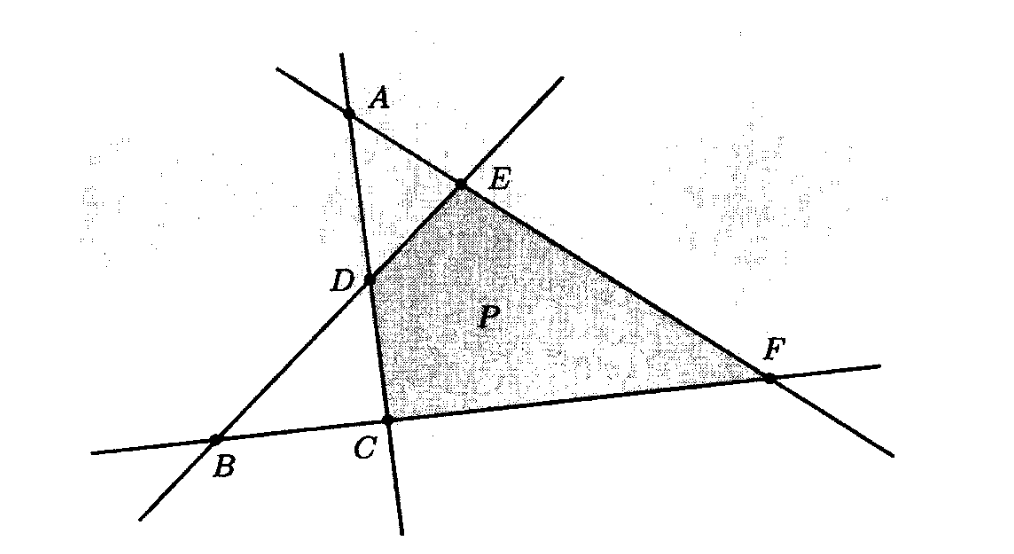
\includegraphics[width=0.5\textwidth]{fig/BT-fig2.7.png}
    \caption{Figure~2.7 in {\em Introduction To Linear Optimization} by Bertsekas and Tsitsiklis. The figure illustrates a polyhedral set $P\subset\rr^2$ where $A, B, C, D, E, F$ are all basic solutions to $P$ but only $C, D, E, F$ are basic feasible solutions. Every pair on the same line is a pair of adjacent basic solutions to $P$. }
    \label{fig: basic solution and adjacency}
\end{figure}

We should remind reader junior readers that the term ``basic'' stands for the adjective for ``basis'', which states that the solution is generated by a chosen linear algebraic basis. Observe that these two definitions, and the definition for an extreme point, are the same object in three different aspects. Before unifying the three characterizations of a polyhedral corner, it is worth reflecting on the logical architecture of our exposition. In Chapter~\ref{chapter: polyhedral geometry}, we established the fundamental equivalence between extreme points and basic feasible solutions ($\text{extreme point} \iff \text{basic feasible solution}$). This ordering is both deliberate and necessary: extreme points (geometric/topological) and basic feasible solutions (algebraic/algorithmic) are intrinsic to the polyhedron $P$ itself, depending solely on its defining constraint system without reference to an objective function. By isolating this intrinsic geometry-to-algebra bridge first in Theorem~\ref{thm: extreme points part 1}, we established a constructive computational skeleton for $P$. In this section, we introduce the extrinsic optimization perspective: the notion of a vertex defined relative to an optimization objective $\inner{\bmc, \cdot}$; and close the loop to synthesize all three viewpoints into one unified equivalence

\begin{theorem}
For a polyhedral set $P\subset \rr^{n}$ and a point $\bmx\rast \in \rr^{n}$. The following are equivalent. 
\begin{itemize}[noitemsep]
\item The point $\bmx\rast$ is a vertex in $P$. 
\item The point $\bmx\rast$ is an extreme point in $P$. 
\item The point $\bmx\rast$ is a basic feasible solution to $P$. 
\end{itemize}
\end{theorem}
\begin{proof}
Observe that Theorem~\ref{thm: extreme points part 1} is the proof for the point being an extreme point if and only if it is a basic feasible solution to $P$. We first show that a point $\bmx\rast$ is a vertex in $P$ implies that it is an extreme point in $P$; finally, we show that a point is a basic feasible solution to $P$ implies that it is a vertex in $P$. 

Suppose that $\bmx\rast\in P$ is a vertex. By definition, there exists $\bmc\in\rr^{n}$ such that for all $\bmx\in P\setminus\{\bmx\rast\}$, we have that $\inner{\bmc, \bmx\rast} > \inner{\bmc, \bmx}$. This says, for any two other points $\bmu, \bmw\in P$ and any $\alpha \in (0, 1)$, we have that 
\[ \inner{\bmc, \bmx\rast} > \alpha \inner{\bmc, \bmu}  + (1-\alpha) \inner{\bmc, \bmw}. \] 
Thus, there are no lines with endpoints in $P$ that contain $\bmx\rast$. 

Suppose that $\bmx\rast\in P$ is a basic feasible solution to $P$. Without loss of generality, we may assume $\bma_1, \bma_2, \dots, \bma_r$ are linear independent active constraints so that $\inner{\bma_j, \bmx\rast} = b_j$ that attains the bounds $b_j$, for $j\in\{1, 2, \dots, r\}$. We define a vector $\bmc = \sum_{i = 1}^m \bma_j$. Since the constraints are active, we have that  $\inner{\bmc, \bmx\rast} = \sum_{i = 1}^m  b_j$. By the linear indepdence, $\bmx\rast$ is the unique solution so that $\inner{\bma_j, \bmx\rast} = b_j$ for all $j\in\{1,2,\dots, r\}$ and, for any other $\bmx \in P\setminus\{\bmx\rast\}$, we have that $ \inner{\bma_j, \bmx\rast} > \inner{\bma_j, \bmx}$; this follows the definition of $\bmx\rast$ is a vertex in $P$. 
\end{proof}

%\begin{theorem}[Fundamental Theorem of Linear Programming]
%Consider the linear programming problem $\max_{\bmx} \inner{\bmc, \bmx}$ subject to $A\bmx\leq \bmb$, the optimal value $\bmx\rast$ occurs on the polyhedral set $\{\bmx: A\bmx = \bmb\}$. 
%\end{theorem}

%We remark on the choice of indices and rows; observe that $I_m = I_m^\top$. 
%\[A = \bmat{M\\ -M \\ -I_{m}} = 
%\left[\begin{array}{cccccc}
%| & | &  & | & & | \\ 
%\bmc_1& \bmc_2 & \dots & \bmc_k & \dots & \bmc_m\\
%| & | &  &| & & | \\ \hline
%| & | &  & | & & | \\ 
%-\bmc_1& -\bmc_2 & \dots & -\bmc_k & \dots & -\bmc_m\\
%| & | &  &| & & | \\ \hline
%| & | &  & | & & | \\ 
%-\bm\chi_1& -\bm\chi_2 & \dots & -\bm\chi_k & \dots & -\bm\chi_m\\
%| & | &  & | & & | \\ 
%\end{array}\right] 
%\]
%Next, we choose from $M$ a set of linearly independent rows, which are guaranteed by the fundamental theorem of linear algebra, and append a set of 
% 




\bibliographystyle{unsrtnat}
\bibliography{ref}
\end{document}